\documentclass[preprint,12pt]{elsarticle}

\usepackage[T1]{fontenc}
\usepackage{lmodern}
\usepackage{microtype}
\usepackage{amsmath,amssymb,amsthm,mathtools,bm}
\usepackage{booktabs,multirow,array,tabularx,longtable}
\usepackage{algorithm}
\usepackage{algpseudocode}
\usepackage{tikz}
\usepackage{pgfplots}
\usepackage{xcolor}
\usepackage{graphicx}
\usepackage{subcaption}
\usepackage{enumitem}
\usepackage{xurl}
\usepackage[hidelinks]{hyperref}
\usepackage[capitalize,noabbrev]{cleveref}
\usetikzlibrary{arrows.meta,positioning,calc,fit,backgrounds,shapes.geometric,shapes.symbols,decorations.pathreplacing,patterns,matrix,shadows.blur}
\pgfplotsset{compat=1.18}
\definecolor{shblue}{HTML}{2F6B9A}
\definecolor{shbluefill}{HTML}{DCECF7}
\definecolor{shorange}{HTML}{C65D20}
\definecolor{shorangefill}{HTML}{FBE3D3}
\definecolor{shgreen}{HTML}{2E7D5B}
\definecolor{shgreenfill}{HTML}{DDF1E7}
\definecolor{shpurple}{HTML}{6C4AA1}
\definecolor{shpurplefill}{HTML}{E9E0F5}
\definecolor{shgray}{HTML}{5F6770}
\definecolor{shgrayfill}{HTML}{EEF0F2}
\tikzset{
  sh/component/.style={draw=shblue,fill=shbluefill,rounded corners=2pt,thick,minimum width=25mm,minimum height=11mm,align=center,font=\small},
  sh/source/.style={draw=shgray,fill=shgrayfill,rounded corners=2pt,thick,minimum width=22mm,minimum height=10mm,align=center,font=\small,pattern=north east lines,pattern color=gray!25},
  sh/defense/.style={draw=shgreen,fill=shgreenfill,rounded corners=2pt,thick,minimum width=27mm,minimum height=11mm,align=center,font=\small},
  sh/attack/.style={draw=shorange,fill=shorangefill,diamond,aspect=2.2,thick,align=center,font=\small},
  sh/theory/.style={draw=shpurple,fill=shpurplefill,rounded corners=2pt,thick,minimum width=28mm,minimum height=10mm,align=center,font=\small},
  sh/infrastructure/.style={draw=shgray,fill=shgrayfill,rounded corners=2pt,thick,minimum width=25mm,minimum height=10mm,align=center,font=\small},
  sh/flow/.style={-{Latex[length=2.2mm]},thick,draw=shblue,shorten >=2pt,shorten <=2pt},
  sh/secureflow/.style={-{Latex[length=2.2mm]},thick,draw=shgreen,shorten >=2pt,shorten <=2pt},
  sh/attackflow/.style={-{Latex[length=2.2mm]},thick,dashed,draw=shorange,shorten >=2pt,shorten <=2pt},
  sh/control/.style={-{Latex[length=2mm]},semithick,densely dotted,draw=shgray,shorten >=2pt,shorten <=2pt},
  sh/label/.style={midway,fill=white,inner sep=1.5pt,font=\scriptsize,align=center},
  sh/group/.style={draw=shgray,dashed,rounded corners=4pt,inner sep=5pt}
}


\newtheorem{definition}{Definition}
\newtheorem{assumption}{Assumption}
\newtheorem{lemma}{Lemma}
\newtheorem{proposition}{Proposition}
\newtheorem{theorem}{Theorem}
\newtheorem{corollary}{Corollary}
\newtheorem{remark}{Remark}
\newcommand{\SH}{\textsc{SecretHandle}}
\newcommand{\Enter}{\ensuremath{\mathsf{Enter}}}
\newcommand{\Mint}{\ensuremath{\mathsf{Mint}}}
\newcommand{\Resolve}{\ensuremath{\mathsf{Resolve}}}
\newcommand{\Redact}{\ensuremath{\mathsf{Redact}}}
\newcommand{\Reject}{\ensuremath{\mathsf{Reject}}}
\newcommand{\Adv}{\ensuremath{\mathsf{Adv}}}
\newcommand{\Match}{\ensuremath{\mathsf{Match}}}
\newcommand{\View}{\ensuremath{\mathsf{View}}}
\newcommand{\Real}{\ensuremath{\mathsf{Real}}}
\newcommand{\Ideal}{\ensuremath{\mathsf{Ideal}}}
\newcommand{\bits}{\{0,1\}}
\newcommand{\sample}{\xleftarrow{\$}}
\crefname{assumption}{assumption}{assumptions}
\Crefname{assumption}{Assumption}{Assumptions}
\crefname{proposition}{proposition}{propositions}
\Crefname{proposition}{Proposition}{Propositions}
\setlength{\emergencystretch}{2em}
\renewcommand{\topfraction}{0.92}
\renewcommand{\bottomfraction}{0.85}
\renewcommand{\textfraction}{0.06}
\renewcommand{\floatpagefraction}{0.82}
\setcounter{topnumber}{4}
\setcounter{bottomnumber}{3}
\setcounter{totalnumber}{6}

\journal{Elsevier journal manuscript}

\begin{document}
\begin{frontmatter}

\title{SecretHandle: OS-Minted, Destination- and Task-Bound Opaque Secrets for Android Mobile AI Agents}

\author[inst1]{Anonymous Author(s)}
\affiliation[inst1]{organization={Institution withheld for review}, city={City}, country={Country}}

\begin{abstract}
Mobile graphical-user-interface agents must often use a one-time password, credential, address, phone number, or payment identifier to finish a task. Existing agents normally place the value in a screenshot, accessibility tree, prompt, or action argument, so an injected instruction can convert task authority into disclosure or redirection. We present \SH, an Android design for \emph{usable but invisible} secrets. A privileged service mints an opaque, authenticated handle at an authoritative OS source---the SMS or notification pipeline, Credential Manager, clipboard, or wallet---before the raw value reaches the agent. The handle carries a secret type, a task identifier, a destination predicate over package, origin, and field class, and a type-specific lifecycle. The agent observes the handle and issues \texttt{ENTER(handle)} toward a UI node; the OS resolves the value only after authenticating the handle, validating the task and target, enforcing expiry, use count, and confirmation policy, and reserving the handle against races. An observation redactor then masks the resolved field in accessibility and pixel channels.

We formalize mint, resolve, consume, expire, revoke, and redact as a transition system. Under an uncompromised reference monitor, authentic target identity, complete modeled-channel redaction, and a secure message authenticator, we prove conditional properties for agent-view non-disclosure, destination confinement, handle unforgeability, and single-use replay safety. The analysis deliberately excludes semantic misuse inside an allowed destination and side channels outside the modeled observation boundary. We implement an on-device Android prototype and evaluate it across OTP forwarding, destination redirection, replay, and race attacks against Claude Sonnet~4.6-driven Mobile-Agent v3.5 agents. \SH{} achieves 0.00 observed exposure ($0/30$, Wilson $[0.00, 0.11]$) versus 0.97 for unprotected agents ($29/30$), eliminates destination redirection leakage ($0/30$ versus $30/30$ for unbound placeholders), and imposes sub-microsecond vault resolution latency ($0.13\,\mu\text{s}$) with zero concurrency anomalies.

\end{abstract}

\begin{keyword}
mobile AI agents \sep Android security \sep opaque capabilities \sep destination binding \sep one-time passwords \sep prompt injection \sep observation redaction \sep trusted input
\end{keyword}

\end{frontmatter}

\begin{highlights}
\item Secret handles are minted inside Android at authoritative sources, before an agent can observe a raw secret.
\item Each opaque handle is bound to a task and destination and carries a type-specific lifetime and use policy.
\item The OS resolves \texttt{ENTER(handle)} locally and redacts the resulting field from later agent observations.
\item A transition-system analysis states conditional non-disclosure, confinement, unforgeability, and replay properties.
\item A reproducible AOSP evaluation protocol is provided; no placeholder curve is reported as an empirical result.
\end{highlights}

\section{Introduction}
\label{sec:introduction}

Mobile agents increasingly operate applications by reading screenshots or accessibility trees and producing taps, swipes, and text-entry actions. Systems and benchmarks such as AppAgent, Mobile-Agent, AutoDroid, AndroidWorld, AndroidEnv, Android in the Wild, and SPA-Bench show why this interface is attractive: it reaches applications without requiring each developer to expose an agent-specific API \cite{zhang2023appagent,wang2024mobileagent,wen2023autodroid,rawles2024androidworld,toyama2021androidenv,rawles2023aitw,chen2024spabench}. The same interface collapses a security boundary. If a code or credential is visible enough for an agent to copy, it is visible enough for a compromised model, cloud endpoint, injected webpage, malicious notification, or logging layer to exfiltrate.

The risk is not hypothetical at the level of mechanism. Indirect prompt injection lets untrusted content compete with the user's instruction \cite{greshake2023indirect,zhan2024injecagent,debenedetti2024agentdojo}; GUI-specific studies demonstrate that visually embedded or third-party content can steer agents toward privacy violations \cite{chen2025fineprint,liao2024eia,chen2025aeia}. A recent mobile study exercises multi-app adversarial workflows and cross-app data exfiltration \cite{du2025mobileattacks}. These results do not imply that every agent or every task fails, but they establish that a secret exposed to the planning loop is inside the attack surface.

Prompt filtering cannot provide the required invariant. A detector may miss a sensitive span; a placeholder may be substituted into the wrong field; and a model that never reads a value may still direct a local resolver to disclose it at an attacker-chosen destination. Mobile placeholder privacy is an important step: the closest design transforms sensitive screen content into type-preserving placeholders and mediates actions locally \cite{zhao2026anonymization}. AutoDroid also includes prompt-side substitution as part of mobile task automation \cite{wen2023autodroid}. Both motivate an abstraction boundary, but a security claim that begins after screen capture depends on detection coverage and does not itself bind the eventual value to the app, web origin, task, or field that is authorized to receive it.

This paper asks a narrower systems question: \emph{can Android let an untrusted agent use a secret without ever giving the agent the secret or a transferable bearer copy?} Our answer is \SH, an OS-minted opaque capability. Android already contains authoritative source points and relevant enforcement primitives: SMS Retriever routes app-associated verification messages \cite{androidSmsRetriever}; Autofill and Credential Manager mediate user data for app fields \cite{androidAutofill,androidCredentialManager,androidAutofillServices}; Android 15 redacts detected OTP content from untrusted notification listeners and remote screen sharing \cite{android15privacy}; and hardware-backed Keystore, key attestation, and Protected Confirmation support protected keys and high-assurance confirmation \cite{androidKeystore,androidKeyAttestation,androidProtectedConfirmation}. \SH\ connects these ideas to the accessibility-agent action path.

At mint time, the trusted source pipeline gives the SecretHandle service a raw value, a type, provenance, and the narrowest defensible destination. The service stores the value in OS-private memory or sealed storage and returns a randomized identifier plus an authenticator. The agent receives only a typed description such as \texttt{OTP\#7 expires in 43s; destination: com.example.bank/login\_otp}. To act, it sends \texttt{ENTER(OTP\#7)} and a target-node token. The resolver authenticates the handle, verifies the current task, package, WebView origin when trustworthy, field class, time, remaining uses, and confirmation rule, atomically reserves the record, and injects the value below the agent's observation boundary. The subsequent accessibility tree and screenshot contain a masked projection rather than the value.

Destination binding resembles audience restriction, not encryption for the model. OAuth resource indicators prevent a token intended for one resource from being replayed at another \cite{rfc8707}; DPoP additionally constrains a token to a presenter key \cite{rfc9449}. WebAuthn scopes credentials to relying parties \cite{webauthn3}. \SH\ applies a related principle to local UI data flow: possession of a handle is insufficient unless the OS-observed target and task match the handle policy. This analogy guides the design but does not make an OAuth token, passkey, or payment token an empirical baseline for Android text entry.

\subsection{Contributions}

This manuscript makes five scoped contributions.

\begin{enumerate}[leftmargin=*]
  \item It defines an OS-minted secret-handle abstraction for Android in which the raw value is intercepted at an authoritative source and represented to a mobile AI agent by a non-semantic, authenticated capability.
  \item It designs a destination- and task-bound resolver for \texttt{ENTER(handle)} with atomic use reservation, typed lifecycles, optional protected confirmation, and explicit failure semantics. The destination includes package identity and may include a trustworthy web origin and field class; this granularity is a policy decision, not assumed ground truth.
  \item It integrates observation-side redaction across accessibility and screenshot channels and identifies the closure conditions required to keep a just-entered value out of the next planning observation.
  \item It supplies a formal transition system and conditional proofs for non-disclosure in the modeled agent view, destination confinement, reduction-style unforgeability, and single-use/expiry safety. The results do not claim to stop malicious actions that remain within an authorized destination.
  \item It gives an implementation blueprint and preregistration-style evaluation plan for AOSP devices, login/2FA/checkout applications, real mobile agents, redirection and replay attacks, ablations, leakage instrumentation, and latency measurement. No unmeasured number is presented as a result.
\end{enumerate}

\subsection{Scope and paper organization}

The trusted computing base includes the Android kernel and relevant framework services, the source adapters, the SecretHandle store and resolver, the redaction paths, and protected key operations. The agent, model provider, third-party content, and ordinary applications are untrusted. A compromised OS, a covert camera, timing leakage, or a malicious authorized destination is outside the central guarantee and is discussed in \cref{sec:limitations}. The rest of the paper separates prior work (\cref{sec:related}), notation and platform context (\cref{sec:preliminaries}), the model and properties (\cref{sec:system,sec:problem}), the design and algorithms (\cref{sec:method,sec:algorithm}), formal analysis (\cref{sec:theory}), and the planned evaluation (\cref{sec:experiments}).

\section{Related work and novelty boundary}
\label{sec:related}

\subsection{Mobile GUI agents and benchmarks}

AppAgent uses multimodal interaction and experience learned through exploration or demonstrations \cite{zhang2023appagent}. Mobile-Agent emphasizes vision-centric perception without relying on app XML, while Mobile-Agent-v2 separates planning, decision, and reflection and Mobile-Agent-v3 broadens the framework across GUI environments \cite{wang2024mobileagent,wang2024mobileagentv2,ye2025mobileagentv3}. AutoDroid combines dynamic app analysis, UI representation, memory, and query optimization for Android task automation \cite{wen2023autodroid}. ScreenAgent and OSWorld expand the design and evaluation space for visual computer control \cite{niu2024screenagent,xie2024osworld}.

Android in the Wild provides large-scale demonstrations; AndroidEnv provides an interactive reinforcement-learning platform; AndroidWorld supplies reproducible state setup and programmatic task checks; and SPA-Bench integrates multiple smartphone agents and metrics \cite{rawles2023aitw,toyama2021androidenv,rawles2024androidworld,chen2024spabench}. These works establish observation and action interfaces that \SH\ must support. They do not claim an OS primitive for using an OTP or credential while withholding it from the agent. Moreover, AndroidWorld's standard applications avoid login-dependent tasks, which is why the proposed evaluation adds purpose-built, open authentication and checkout flows rather than claiming existing benchmark coverage.

\subsection{Placeholders and inference-time privacy}

The closest prior direction is privacy-preserving transformation of agent-visible content. Anonymization-Enhanced Privacy Protection for Mobile GUI Agents detects sensitive content, replaces it with type-preserving placeholders, transforms multiple UI representations, and resolves certain local interactions through a proxy \cite{zhao2026anonymization}. This demonstrates that semantic placeholders can preserve task utility. \SH\ changes the trust boundary in two ways: the handle is minted at a source that already owns or receives the value, so protection of integrated sources does not depend on finding the value after rendering; and use is authorized against an OS-observed destination rather than merely replacing a placeholder at a requested index.

Text and prompt privacy systems address a neighboring boundary. Casper detects and removes sensitive prompt content locally \cite{chong2024casper}; PAPILLON coordinates local and remote models for privacy-conscious delegation \cite{siyan2025papillon}; PrivacyRestore removes privacy spans and transmits a restoration representation in a client-server inference design \cite{zeng2025privacyrestore}; and resource-aware work estimates when sanitization will harm utility \cite{carpentier2024preempting}. These techniques can reduce cloud disclosure, but a mobile agent still needs a trusted actuation path when the hidden value must be entered into an application. We therefore treat sanitization as complementary and do not cite it as evidence for destination confinement.

\subsection{Prompt injection, agent isolation, and information flow}

Indirect prompt injection is an architectural risk when an agent interprets untrusted data as instructions \cite{greshake2023indirect}. InjecAgent and AgentDojo provide structured tests of attacks and defenses for tool-integrated agents \cite{zhan2024injecagent,debenedetti2024agentdojo}. Fine-print and environmental injection studies extend this concern to visual and GUI environments \cite{chen2025fineprint,liao2024eia,chen2025aeia}; mobile-agent experiments show that third-party channels can participate in realistic adversarial workflows \cite{du2025mobileattacks}.

Architectural defenses seek guarantees outside the language model. CaMeL extracts control and data flow from a trusted query and uses capabilities at tool calls \cite{debenedetti2025camel}. Fides assigns confidentiality and integrity labels in a formal planner model \cite{costa2025fides}. Progent enforces privilege policies for agents \cite{shi2025progent}. IsolateGPT separates apps and their interactions, while AirGapAgent limits task context to reduce disclosure under context hijacking \cite{wu2025isolategpt,bagdasarian2024airgap}. \SH\ shares the premise that a vulnerable model should not be the final policy authority. Its distinct object is a value that must cross from an OS source into a concrete UI field without crossing the planner's observation boundary.

\subsection{Capabilities, mobile information flow, and Android mediation}

Capabilities are unforgeable tokens of authority rather than descriptive names alone \cite{dennis1966semantics}. Least privilege, complete mediation, fail-safe defaults, and economy of mechanism remain useful design criteria \cite{saltzer1975protection}. Capsicum demonstrates a practical capability model for compartmentalizing commodity UNIX applications \cite{watson2010capsicum}. \SH\ is not a general-purpose object-capability OS; it uses a narrow capability-shaped record for one actuation right, including explicit attenuation by destination, task, time, and use count.

Android security research has shown both platform mediation and its limits. Android Permissions Demystified measured the mapping between API behavior and permissions \cite{felt2011permission}. Fine-grained mandatory access-control work and SEApp illustrate the value and engineering cost of adding policies below applications \cite{bugiel2013flexible,rossi2021seapp}. TaintDroid tracks sensitive flows dynamically from sources to sinks, while DroidScope reconstructs OS and runtime semantics for analysis \cite{enck2010taintdroid,yan2012droidscope}. \SH\ differs from taint tracking: it aims to prevent the raw value from entering an untrusted agent-visible representation, then authorizes one explicit sink. Tainting remains useful as an evaluation oracle for detecting accidental flows.

\subsection{Authentication and bound tokens}

HOTP and TOTP standardize common one-time-password constructions \cite{rfc4226,rfc6238}; NIST guidance describes authenticator and lifecycle considerations \cite{nist80063b}. These standards define or govern codes, not how an accessibility agent can enter a code without seeing it. Android's SMS Retriever can route a verification message associated with an app, and OTP Autofill can mediate user-approved filling \cite{androidSmsRetriever,androidAutofillServices}. Credential Manager and Autofill are primarily app- and user-driven platform interfaces \cite{androidCredentialManager,androidAutofill}. \SH\ reuses their source knowledge where available but adds an agent action that never returns the value to the agent.

Audience restriction in OAuth prevents a token intended for one protected resource from being replayed at another, and DPoP adds proof-of-possession sender constraint \cite{rfc8707,rfc9449,rfc9700}. WebAuthn scopes public-key credentials to relying parties \cite{webauthn3}. These systems motivate narrow binding and explicit validation. Their network principals and protocols differ from a package/origin/field target inside Android; consequently the paper claims a design analogy, not protocol equivalence.

\subsection{Novelty statement}

Within the verified literature above, we did not find a system that simultaneously (i) mints an agent-facing opaque handle at an Android authoritative source before screen exposure; (ii) binds resolution to the current task and OS-observed UI destination; (iii) enforces a type-specific lifecycle; and (iv) closes both accessibility and pixel observation after entry. This is a bounded literature statement, not a claim of exhaustive priority. The closest mobile-placeholder work is newer than the original concept and materially narrows the novelty boundary; any submission must re-run the search and compare implementations and threat models in detail.

\section{Platform background and notation}
\label{sec:preliminaries}

\subsection{Android observation and actuation}

An accessibility-based agent typically obtains a screenshot and a structured tree containing nodes, bounds, roles, text, content descriptions, and action affordances. Android accessibility services are explicitly privileged components that can observe events and act on behalf of users \cite{androidAccessibility}. A screenshot-only agent may omit the tree, while a hybrid agent aligns visual regions with nodes. In either case, ordinary text entry exposes a string to at least the action-producing process and frequently to logs or prompts.

Android Autofill has a different interaction pattern. The framework connects a client view, the system, and an Autofill service; the client exposes structure and accepts a selected dataset \cite{androidAutofill,androidAutofillServices}. Credential Manager aggregates passkeys, passwords, and federated sign-in credentials through app requests and user-facing selectors \cite{androidCredentialManager}. These mechanisms are useful precedents because the OS mediates sensitive data, but an autonomous accessibility agent generally cannot assume that the target app has initiated the appropriate request or that every relevant secret type has a platform provider.

Android already distinguishes some sensitive sources. The SMS Retriever flow delivers an app-associated verification message to a registered app and expects server-side verification \cite{androidSmsRetriever}. User Consent allows a one-time, user-mediated SMS read \cite{androidSmsConsent}. The clipboard sensitivity extra is a rendering hint rather than an access-control guarantee \cite{androidClipboard}. Android 15 adds OTP redaction for many untrusted notification listeners and screen-sharing protections \cite{android15privacy}. \SH\ treats these as source-specific signals and enforcement hooks, not as proof that the unified design already exists.

\subsection{Cryptographic and capability terminology}

Let $\lambda$ denote the security parameter and $F_K:\bits^*\rightarrow\bits^\lambda$ a message authentication function keyed by $K$. The implementation may use an approved HMAC construction \cite{rfc2104} with a non-exportable key in Android Keystore \cite{androidKeystore}; the model needs only existential unforgeability under chosen-message attack for the authenticated handle representation. A capability conveys authority. A printed string that merely looks like a handle is not a capability unless the resolver authenticates it and finds a live server-side record.

We distinguish four identities: package identity $p$, web origin $o$, field class $f$, and task identity $\tau$. A destination policy $d$ is a predicate over a target context rather than necessarily a single tuple. For a native app, $d$ may restrict $p$ and $f$. For a WebView, it may also restrict $o$, but only if the platform can authenticate the displayed document origin. If reliable origin extraction is unavailable, policy must fail closed or require confirmation; it must not silently downgrade to a package-only guarantee.

\begin{table}[htbp]
\centering
\caption{Principal notation. Every symbol used in the core transition system is defined here.}
\label{tab:notation}
\begin{tabularx}{\textwidth}{@{}lX@{}}
\toprule
Symbol & Meaning \\
\midrule
$s\in\mathcal{S}$ & Raw secret value, never intentionally included in the agent view. \\
$q\in\mathcal{Q}$ & Secret type: OTP, credential, identifier, clipboard value, or payment token. \\
$\sigma\in\mathcal{P}$ & Authoritative source and provenance statement. \\
$\tau\in\mathcal{T}$ & Unforgeable or OS-authenticated task identifier. \\
$d\in\mathcal{D}$ & Destination predicate over package, origin, field class, and optional app-defined context. \\
$n\in\bits^\lambda$ & Fresh random handle identifier. \\
$t_i,t_e$ & Issue and expiry times, with $t_i<t_e$. \\
$u\in\mathbb{N}$ & Remaining successful-use budget. \\
$c\in\mathcal{C}$ & Confirmation policy, e.g., none, biometric, or Protected Confirmation. \\
$H=(n,q,\sigma,d,\tau,t_i,t_e,u,c)$ & Authenticated handle metadata. \\
$a=F_K(\mathsf{enc}(H))$ & Handle authenticator. \\
$h=(n,q,a)$ & Compact agent-visible handle; non-sensitive display metadata may accompany it. \\
$x=(p,o,f,v)$ & Resolver-authenticated target context for node token $v$. \\
$\Omega$ & Trusted SecretHandle store mapping $n$ to secret and state. \\
$\View_A(\pi)$ & Agent-visible projection of execution trace $\pi$. \\
$\ell$ & Explicit leakage allowed by the interface: type, coarse destination label, age/expiry, and status. \\
\bottomrule
\end{tabularx}
\end{table}

\subsection{Lifecycle classes}

Lifecycle is part of the authority, not advisory metadata. OTP handles default to one successful use and a short TTL matched to the issuer's validity window. Identifier handles may permit multiple uses only inside the same task and destination set. Credential handles are scoped to a relying app or origin and normally require a platform credential-selection event. Payment-class handles additionally require per-use confirmation. A policy profile may always be tightened after minting; widening a destination or use budget requires a newly authenticated handle and, for sensitive classes, fresh user approval.

\begin{table}[htbp]
\centering
\caption{Default policy profiles. These are design defaults to validate experimentally, not platform measurements.}
\label{tab:profiles}
\footnotesize
\renewcommand{\arraystretch}{1.15}
\begin{tabularx}{\textwidth}{@{}>{\raggedright\arraybackslash}p{1.55cm}>{\raggedright\arraybackslash}p{2.45cm}>{\raggedright\arraybackslash}X>{\raggedright\arraybackslash}p{1.75cm}>{\raggedright\arraybackslash}p{2.35cm}@{}}
\toprule
Type & Source & Binding & Use budget & Confirmation \\
\midrule
OTP & SMS/\allowbreak notification & package + OTP field + task & 1; short TTL & none/\allowbreak user-consent \\
Credential & Credential Manager & package/origin + task & 1 per request & platform selector \\
Identifier & clipboard/\allowbreak profile & package + field class + task & bounded task use & policy dependent \\
Payment & wallet/\allowbreak token provider & package/origin + checkout task & 1 & per-use protected UI \\
\bottomrule
\end{tabularx}
\end{table}

\subsection{Design principles}

The design follows four rules. First, \emph{mint before observation}: a protected source never emits the raw value onto an agent-readable path. Second, \emph{authorize the sink}: the target is checked from trusted framework state, not from the model's textual assertion. Third, \emph{consume atomically}: concurrent calls cannot both pass a single-use check. Fourth, \emph{close the observation loop}: resolving a value is not sufficient if the next tree or screenshot reveals it.

These principles refine least privilege and complete mediation \cite{saltzer1975protection}. They also expose a limitation: a source not integrated with the OS cannot receive detector-independent protection. Such content may still use a detector-based placeholder, but its guarantee must be stated separately.

\section{System and threat model}
\label{sec:system}

\subsection{Entities and trust boundary}

\begin{figure}[htbp]
\centering
\resizebox{0.92\textwidth}{!}{%
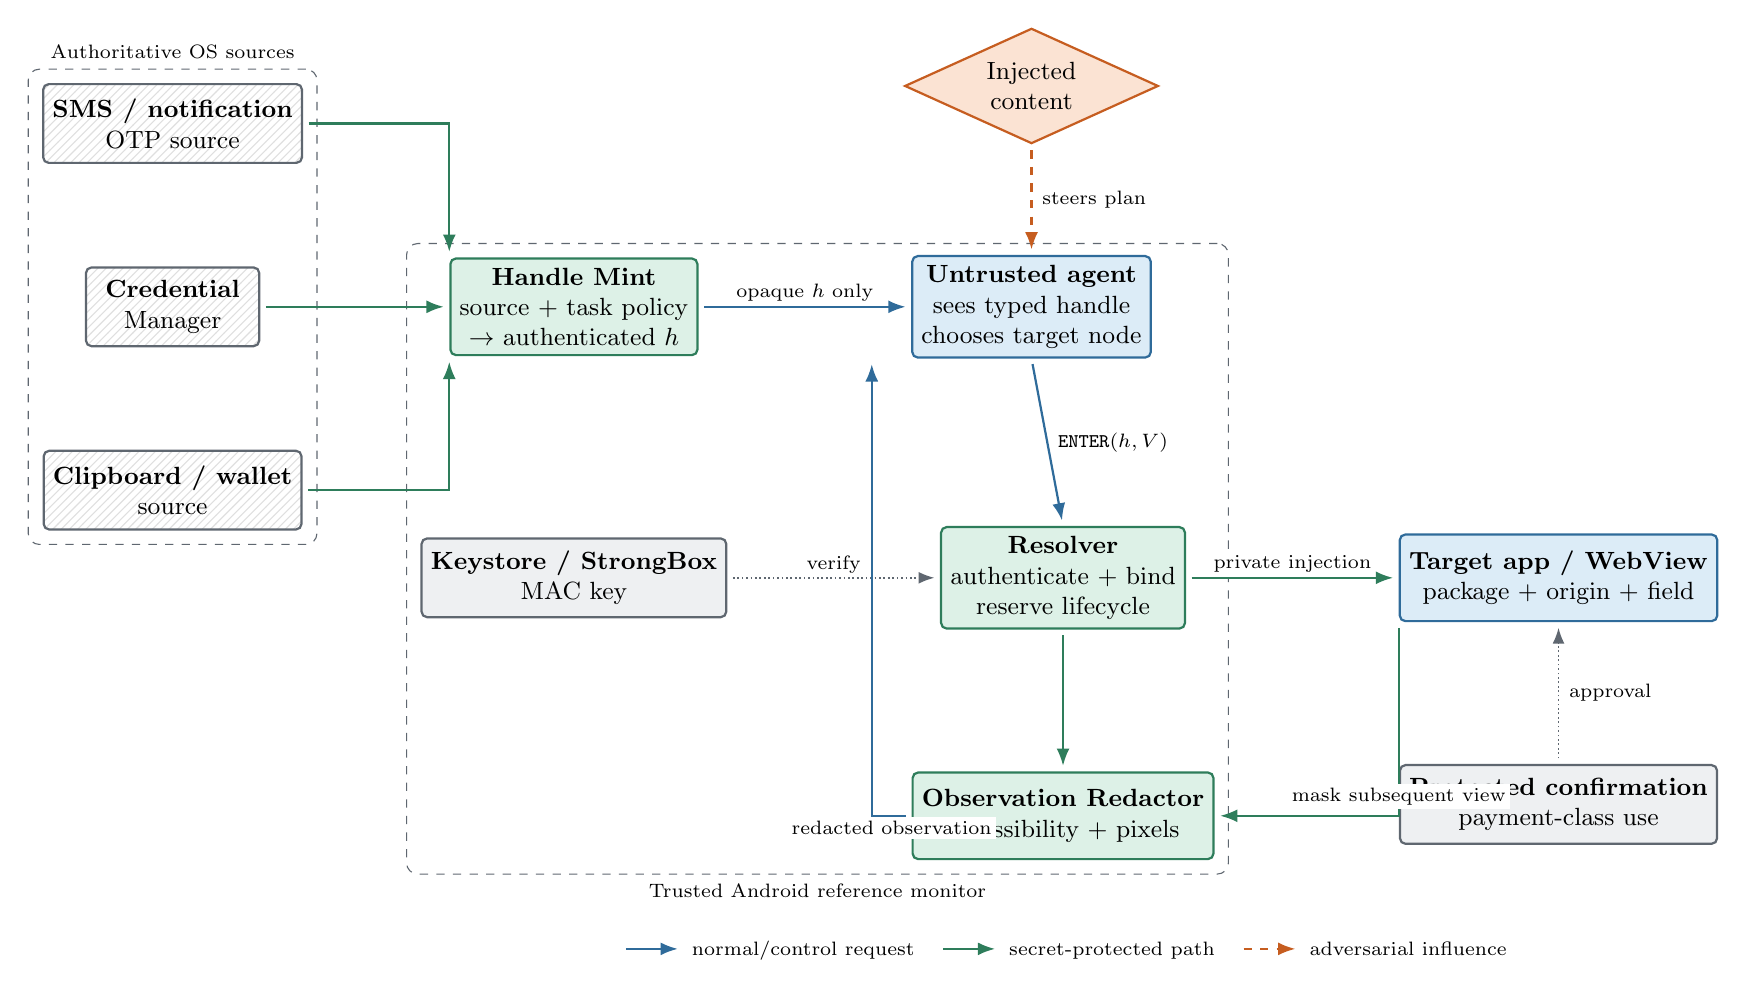
\begin{tikzpicture}[node distance=13mm and 22mm]
\node[sh/source] (sms) {\textbf{SMS / notification}\\OTP source};
\node[sh/source,below=of sms] (cred) {\textbf{Credential}\\Manager};
\node[sh/source,below=of cred] (clip) {\textbf{Clipboard / wallet}\\source};
\node[sh/defense,right=24mm of cred] (mint) {\textbf{Handle Mint}\\source + task policy\\$\rightarrow$ authenticated $h$};
\node[sh/component,right=27mm of mint] (agent) {\textbf{Untrusted agent}\\sees typed handle\\chooses target node};
\node[sh/attack,above=14mm of agent] (attack) {Injected\\content};
\node[sh/infrastructure,below=23mm of mint] (keys) {\textbf{Keystore / StrongBox}\\MAC key};
\node[sh/defense,right=27mm of keys] (resolver) {\textbf{Resolver}\\authenticate + bind\\reserve lifecycle};
\node[sh/component,right=27mm of resolver] (app) {\textbf{Target app / WebView}\\package + origin + field};
\node[sh/defense,below=18mm of resolver] (redactor) {\textbf{Observation Redactor}\\accessibility + pixels};
\node[sh/infrastructure,below=18mm of app] (confirm) {\textbf{Protected confirmation}\\payment-class use};
\draw[sh/secureflow] (sms.east) -| (mint.north west);
\draw[sh/secureflow] (cred.east) -- (mint.west);
\draw[sh/secureflow] (clip.east) -| (mint.south west);
\draw[sh/flow] (mint.east) -- node[sh/label,above] {opaque $h$ only} (agent.west);
\draw[sh/attackflow] (attack.south) -- node[sh/label,right=2pt] {steers plan} (agent.north);
\draw[sh/flow] (agent.south) -- node[sh/label,right=2pt] {\texttt{ENTER}$(h,V)$} (resolver.north);
\draw[sh/control] (keys.east) -- node[sh/label,above] {verify} (resolver.west);
\draw[sh/secureflow] (resolver.east) -- node[sh/label,above] {private injection} (app.west);
\draw[sh/control] (confirm.north) -- node[sh/label,right=2pt] {approval} (app.south);
\draw[sh/secureflow] (resolver.south) -- (redactor.north);
\draw[sh/secureflow] (app.south west) |- node[sh/label,pos=.45] {mask subsequent view} (redactor.east);
\draw[sh/flow] (redactor.west) -| node[sh/label,pos=.25,below] {redacted observation} ([xshift=-5mm]agent.south west);
\begin{scope}[on background layer]
\node[sh/group,fit=(sms)(cred)(clip),label={[font=\scriptsize]above:Authoritative OS sources}] {};
\node[sh/group,fit=(mint)(keys)(resolver)(redactor),label={[font=\scriptsize]below:Trusted Android reference monitor}] {};
\end{scope}
\node[below=9mm of redactor,font=\scriptsize,align=left] (legend) {\tikz\draw[sh/flow] (0,0)--(.8,0); normal/control request\quad
\tikz\draw[sh/secureflow] (0,0)--(.8,0); secret-protected path\quad
\tikz\draw[sh/attackflow] (0,0)--(.8,0); adversarial influence};
\end{tikzpicture}%
}
\caption{SecretHandle architecture. The raw value travels only from an authoritative source through the trusted mint/resolver path to an accepted destination. The agent receives an opaque handle and a redacted post-entry view. Colors and line styles distinguish ordinary, protected, and adversarial flows.}
\label{fig:architecture}
\end{figure}


The trusted computing base (TCB) contains the Android kernel, the relevant portion of \texttt{system\_server}, the SecretHandle service, source adapters, the resolver and input-dispatch integration, accessibility and screenshot redactors, and the keystore operation used to authenticate records. A payment confirmation path may place the confirmation UI and key authorization inside a TEE; Android Protected Confirmation is optional at the device level and therefore must be detected rather than assumed \cite{androidProtectedConfirmation}.

The agent process, local or remote model, model provider, agent memory, ordinary applications, rendered web content, notifications not authenticated by a protected source, and app-supplied labels are untrusted. A target application may be honest, malicious, or confused. SecretHandle's destination property says whether a handle may be resolved at a target identity; it does not prove that an allowed app will subsequently use the value honestly.

The user authorizes a task and may approve sensitive mint or resolve events. The task broker gives the service a task identifier $\tau$ and an initial destination policy. The mechanism assumes $\tau$ cannot be chosen or modified by the agent alone. This can be implemented by an OS-signed task token or by state held in the service. The concept document mentions composition with a separate task-capability mechanism; because that artifact is not present, the manuscript specifies the minimum task-token contract independently rather than relying on an unavailable result.

\subsection{Authoritative sources}

An authoritative source is a TCB component or mediated provider that receives the secret before an agent-readable representation and can supply trustworthy provenance. The initial adapters are:

\begin{itemize}[leftmargin=*]
  \item \textbf{SMS/notification OTP adapter.} It observes a verification message in the protected delivery or classification path, derives an app binding when the message or request supports one, and withholds the code from the agent-facing notification. App-hash association is evidence for an app, not evidence for an arbitrary field.
  \item \textbf{Credential Manager adapter.} It mints only after the user selects a credential for a requesting app or origin. The adapter retains the credential material inside the provider/system path and exports a one-use handle.
  \item \textbf{Clipboard adapter.} It mints only for clips explicitly marked or user-designated as sensitive. Because \texttt{EXTRA\_IS\_SENSITIVE} does not itself change clipboard access control \cite{androidClipboard}, SecretHandle must suppress or replace agent-visible clip content in addition to reading the hint.
  \item \textbf{Wallet adapter.} It accepts a token or payment credential from a wallet/provider contract and requires confirmation. Server-side payment tokenization is complementary; the local handle controls which UI destination receives the wallet output.
\end{itemize}

An OCR or named-entity detector is not an authoritative source. It may create a best-effort legacy handle with a visibly weaker assurance label, but such a path is excluded from the detector-independent theorems.

\subsection{Adversary capabilities}

The adversary controls the agent's planning output and may arrange arbitrary untrusted text or pixels in an app, webpage, notification, or message. It can request actions on any node visible to the agent, replay previously observed handles, guess new handle strings, race multiple \texttt{ENTER} calls, switch foreground apps, navigate a WebView, and render a string with the same visual syntax as a handle. It may read all agent inputs, outputs, prompts, tool traces, and application-visible values after legitimate injection if the destination app itself is compromised.

The adversary cannot read TCB memory, forge Android package identity, extract the non-exportable handle-authentication key, modify the resolver's atomic state transition, compromise the trusted display used for Protected Confirmation, or bypass every screenshot/accessibility redaction hook. These are explicit assumptions. A result that depends on them is a conditional system theorem, not an unconditional statement about all Android devices.

\subsection{Security goals}

\begin{figure}[htbp]
\centering
\resizebox{0.92\textwidth}{!}{%
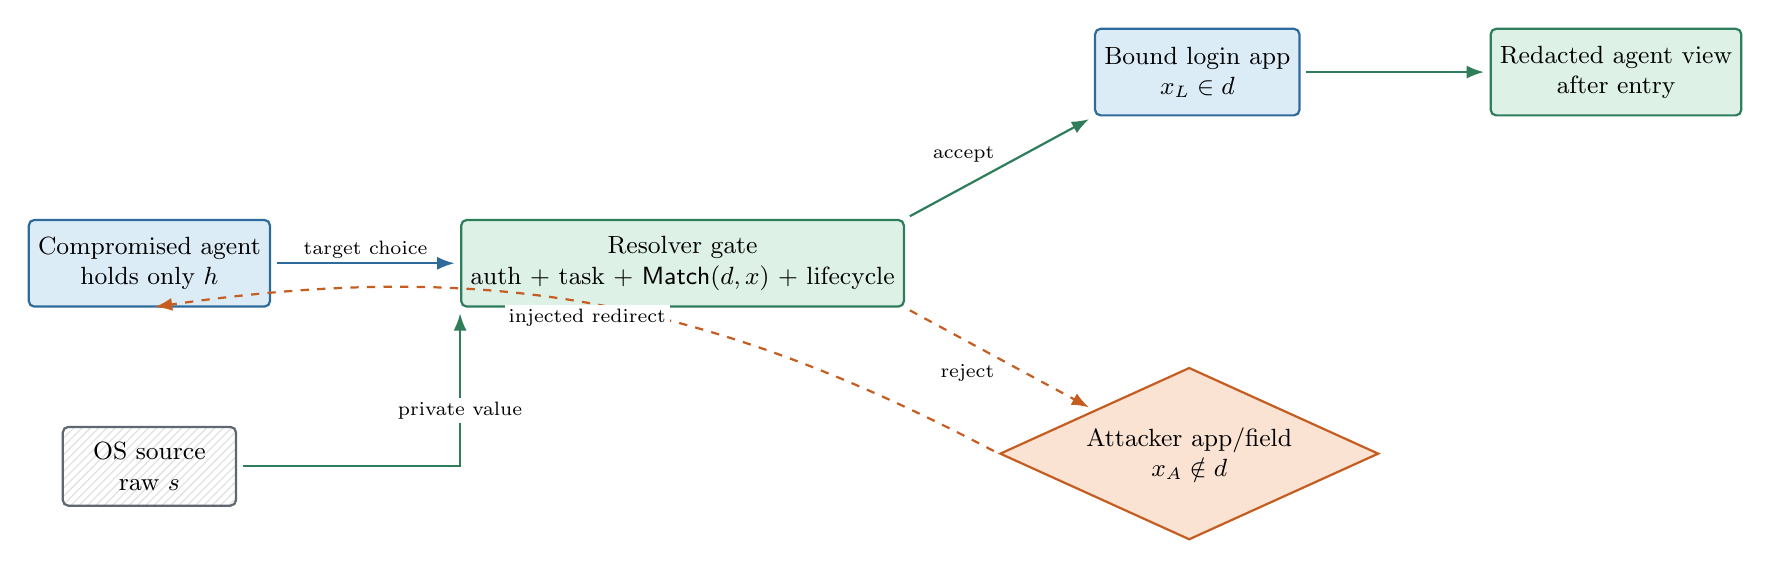
\begin{tikzpicture}[node distance=15mm and 24mm]
\node[sh/component] (agent) {Compromised agent\\holds only $h$};
\node[sh/defense,right=of agent,minimum width=46mm] (gate) {Resolver gate\\auth + task + $\Match(d,x)$ + lifecycle};
\node[sh/source,below=of agent] (secret) {OS source\\raw $s$};
\node[sh/component,above right=13mm and 24mm of gate] (honest) {Bound login app\\$x_L\in d$};
\node[sh/attack,below right=13mm and 24mm of gate] (adv) {Attacker app/field\\$x_A\notin d$};
\node[sh/defense,right=24mm of honest] (mask) {Redacted agent view\\after entry};

\draw[sh/flow] (agent.east) -- node[sh/label,above] {target choice} (gate.west);
\draw[sh/secureflow] (secret.east) -| node[sh/label,pos=.72,below] {private value} (gate.south west);
\draw[sh/secureflow] (gate.north east) -- node[sh/label,above left] {accept} (honest.south west);
\draw[sh/attackflow] (gate.south east) -- node[sh/label,below left] {reject} (adv.north west);
\draw[sh/secureflow] (honest.east) -- (mask.west);
\draw[sh/attackflow] (adv.west) to[bend right=18] node[sh/label,below] {injected redirect} (agent.south);
\end{tikzpicture}%
}
\caption{Threat and control boundary. A compromised agent can choose targets and replay handles, but a handle bound to $d$ is accepted only at a matching target. The figure does not claim protection when the attacker operates inside $d$.}
\label{fig:threat}
\end{figure}


The mechanism targets five goals.

\begin{enumerate}[leftmargin=*]
  \item \textbf{Agent-view non-disclosure:} the modeled agent view reveals only declared leakage $\ell$, not the raw value.
  \item \textbf{Destination confinement:} resolution succeeds only when the trusted target context satisfies the handle's destination predicate and task.
  \item \textbf{Unforgeability:} a string not produced by the mint service is accepted only with negligible probability, subject to authenticator security and identifier entropy.
  \item \textbf{Lifecycle safety:} expired, revoked, consumed, or confirmation-denied handles do not resolve; a single-use handle cannot succeed twice, including under concurrency.
  \item \textbf{Observation closure:} after legitimate entry, the value is masked in subsequent modeled accessibility and pixel observations until the field is cleared or the redaction obligation ends safely.
\end{enumerate}

The utility goal is narrower: authorized login, 2FA, identifier entry, and checkout flows should remain completable with tolerable latency and user burden.

\subsection{Non-goals}

SecretHandle does not detect every prompt injection, determine whether a user-intended task is socially beneficial, stop an authorized bank app from sending an OTP to its server, protect against a compromised kernel, or conceal unavoidable physical effects of task completion. It does not claim that an OTP is phishing-resistant; WebAuthn and passkeys address that authentication problem differently \cite{webauthn3}. It also does not make screenshot-only automation safe when the agent cannot name a stable target node; such agents require a trusted target-selection adapter or user confirmation.

\section{Problem formulation and security definitions}
\label{sec:problem}

\subsection{State and transitions}

The trusted store maps each identifier $n$ to a record
\begin{equation}
\Omega[n]=(s,H,a,z,r),
\label{eq:record}
\end{equation}
where $s$ is the value, $H=(n,q,\sigma,d,\tau,t_i,t_e,u,c)$ is metadata, $a=F_K(\mathsf{enc}(H))$, $z\in\{\mathsf{live},\mathsf{reserved},\mathsf{consumed},\mathsf{expired},\mathsf{revoked}\}$ is lifecycle state, and $r$ is an optional reservation nonce. The visible handle is $h=(n,q,a)$ plus an explicitly non-sensitive label. Storing the complete $H$ server-side prevents the agent from editing a destination even if the display representation is malleable.

The abstract machine supports:
\begin{align}
  (h,\Omega') &\leftarrow \Mint(s,q,\sigma,d,\tau,c,t_i,t_e,u;\Omega), \label{eq:mint}\\
  (y,\Omega') &\leftarrow \Resolve(h,x,\tau',t,\gamma;\Omega), \label{eq:resolve}\\
  O' &\leftarrow \Redact(O,R), \label{eq:redact}
\end{align}
where $x$ is the TCB-derived target context, $\gamma$ is confirmation evidence, $y$ is either an internal injection capability or $\Reject$, $O$ is a raw observation, and $R$ is the active redaction registry. Expiry and revocation are state transitions that never return $s$.

\begin{definition}[Target match]
For trusted context $x=(p,o,f,v)$, $\Match(d,x)=1$ exactly when every mandatory component of destination predicate $d$ accepts the corresponding component in $x$. An unavailable mandatory identity produces $0$, not a wildcard.
\end{definition}

\begin{definition}[Eligible handle]
A record is eligible at time $t$ for task $\tau'$ and target $x$ if its authenticator verifies, its state is live, $t_i\le t<t_e$, $u>0$, $\tau'=\tau$, $\Match(d,x)=1$, and confirmation evidence satisfies $c$.
\end{definition}

\subsection{Observation boundary}

The agent view $\View_A(\pi)$ contains agent-visible screenshots, accessibility trees, handle metadata, action results, timing rounded to the public granularity, and application messages. It excludes TCB memory, sealed storage, protected-confirmation pixels, and the private input buffer between resolver and target. This boundary is intentionally concrete: claiming that ``the agent never sees the value'' without enumerating observations would be unfalsifiable.

Let $\ell(s,H,\pi)$ be allowed leakage. By default it contains $q$, a coarse destination label, issue age bucket, remaining-lifetime bucket, success/failure status, and effects already observable from the task, such as arrival at a logged-in screen. It must not include $s$, a deterministic hash of a low-entropy OTP, value length unless unavoidable, or error codes that distinguish candidate values.

\begin{definition}[Agent-view non-disclosure]
For equal-length secrets $s_0,s_1$ with the same allowed leakage and any probabilistic polynomial-time adversary $\mathcal{A}$ controlling the agent, the distinguishing advantage is
\begin{equation}
\begin{aligned}
\Adv^{\mathsf{nd}}_{\SH,\mathcal{A}}(\lambda)=
\big|&\Pr[\mathcal{A}(\View_A(\Real(s_0)))=1]\\
&-\Pr[\mathcal{A}(\View_A(\Real(s_1)))=1]\big|.
\end{aligned}
\label{eq:nd}
\end{equation}
Non-disclosure holds when this advantage is negligible given equal $\ell$.
\end{definition}

This is a non-interference-style definition with declassified effects. It is stronger than ``the prompt omits the value'' but weaker than preventing inference from all world state. For example, a successful login reveals that the hidden code was accepted; that outcome is intentionally declassified.

\begin{definition}[Destination confinement]
For any trace, if \Resolve\ returns an injection capability containing or referencing $s$ for target $x$ under task $\tau'$, then $\Match(d,x)=1$ and $\tau'=\tau$ for the live record bound to $h$.
\end{definition}

\begin{definition}[Single-use replay safety]
For a handle minted with $u=1$, at most one resolve operation reaches the committed-injection state, even when an adversary schedules an arbitrary number of concurrent calls.
\end{definition}

\subsection{Correctness and availability}

Security is vacuous if the resolver always rejects. Functional correctness requires that an eligible handle aimed at a supported, stable target is injected exactly once unless a platform error occurs, and that the failure is surfaced without revealing $s$. Availability is not absolute: the OS, user, or app may cancel; the target may disappear; a confirmation UI may be unavailable. The evaluation therefore separates policy rejection, platform failure, agent failure, and user denial.

\subsection{Research questions}

The evaluation is organized around six questions:

\begin{description}[leftmargin=1.5cm,style=nextline]
\item[RQ1] Does OS-source minting keep raw values out of all instrumented agent observations and traces?
\item[RQ2] Does destination/task binding prevent injection-driven redirection without blocking legitimate completion?
\item[RQ3] Do lifecycle and atomic reservation prevent replay, expiry bypass, and concurrency races?
\item[RQ4] Does observation redaction prevent post-entry rereading in pixels and accessibility trees?
\item[RQ5] What latency, memory, energy, and user-interaction overheads arise by source and handle type?
\item[RQ6] Which identity ambiguities, unsupported apps, WebViews, keyboards, or OEM modifications cause failure or force a weaker policy?
\end{description}

\section{SecretHandle design}
\label{sec:method}

\begin{figure}[htbp]
\centering
\resizebox{0.78\textwidth}{!}{%
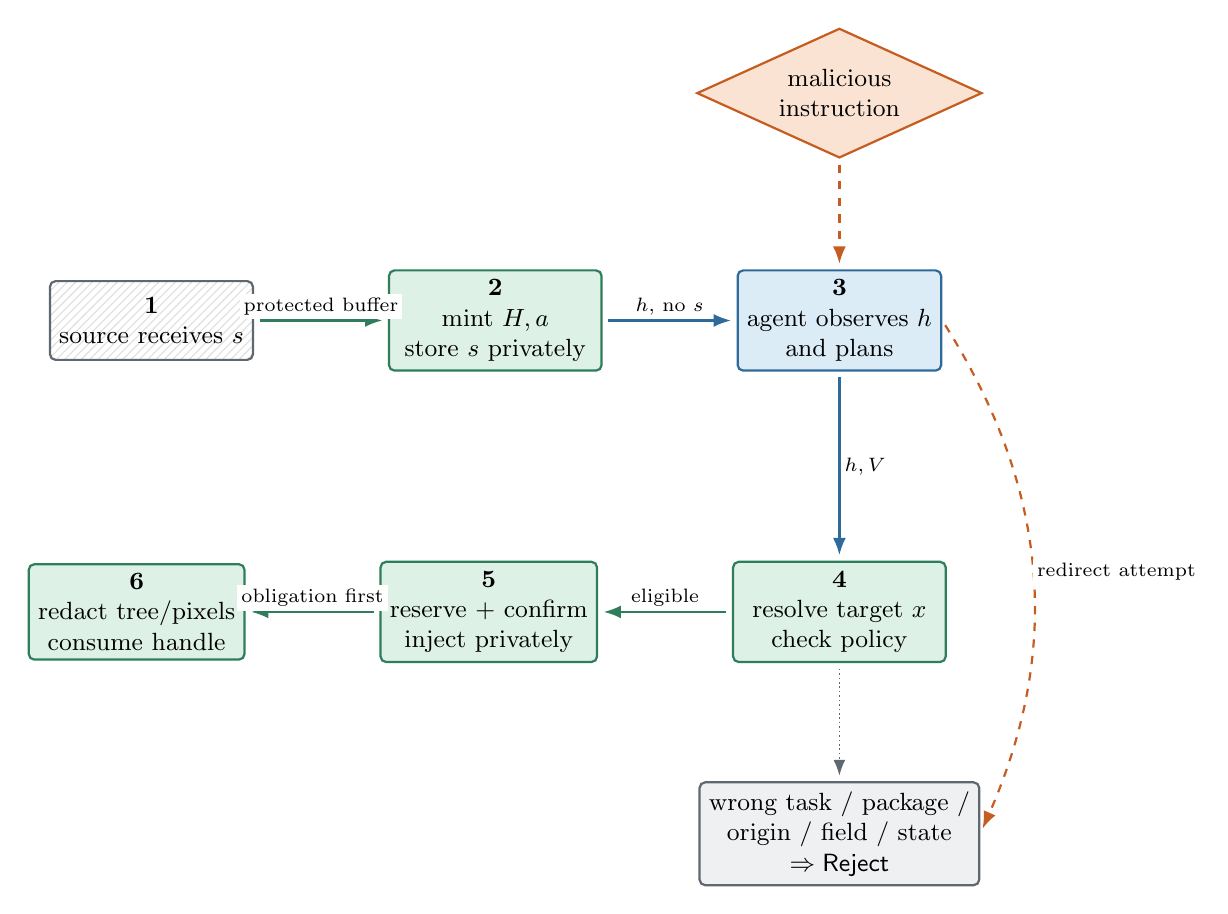
\begin{tikzpicture}[node distance=14mm and 17mm]
\node[sh/source] (s1) {\textbf{1}\\source receives $s$};
\node[sh/defense,right=of s1] (s2) {\textbf{2}\\mint $H,a$\\store $s$ privately};
\node[sh/component,right=of s2] (s3) {\textbf{3}\\agent observes $h$\\and plans};
\node[sh/defense,below=24mm of s3] (s4) {\textbf{4}\\resolve target $x$\\check policy};
\node[sh/defense,left=of s4] (s5) {\textbf{5}\\reserve + confirm\\inject privately};
\node[sh/defense,left=of s5] (s6) {\textbf{6}\\redact tree/pixels\\consume handle};
\draw[sh/secureflow] (s1) -- node[sh/label,above] {protected buffer} (s2);
\draw[sh/flow] (s2) -- node[sh/label,above] {$h$, no $s$} (s3);
\draw[sh/flow] (s3) -- node[sh/label,right] {$h,V$} (s4);
\draw[sh/secureflow] (s4) -- node[sh/label,above] {eligible} (s5);
\draw[sh/secureflow] (s5) -- node[sh/label,above] {obligation first} (s6);
\node[sh/attack,above=14mm of s3] (bad) {malicious\\instruction};
\node[sh/infrastructure,below=15mm of s4] (reject) {wrong task / package /\\origin / field / state\\$\Rightarrow\Reject$};
\draw[sh/attackflow] (bad.south) -- (s3.north);
\draw[sh/attackflow] (s3.east) to[bend left=28] node[sh/label,right] {redirect attempt} (reject.east);
\draw[sh/control] (s4.south) -- (reject.north);
\end{tikzpicture}%
}
\caption{Method pipeline. Security does not depend on the agent recognizing an attack: the resolver checks trusted task and target state, and redaction is installed before private delivery.}
\label{fig:pipeline}
\end{figure}


\subsection{Mint at the authoritative source}

The source adapter invokes a binder interface available only to approved system components. Its request contains the value in a protected buffer, type $q$, provenance $\sigma$, task token, candidate destination evidence, and lifecycle hints. The service validates caller identity and provenance before accepting the value. A third-party app cannot mint an ``OS OTP'' simply by passing a string that looks like a code.

The service derives $d$ using the intersection of independently available constraints. For an SMS Retriever request, it begins with the requesting package association. For Credential Manager, it uses the calling package and verified origin contract. For a task token, it intersects the allowed application set. For the selected target class, it may restrict to an OTP, username, address, or payment field. Intersection is monotonic: each trustworthy source can remove destinations but cannot broaden authority granted by another.

After generating random $n$, the service constructs $H$, computes $a$, stores \cref{eq:record}, wipes the incoming buffer where feasible, and returns $h$. The agent-facing observation replaces the protected content with a stable visual and tree representation. The handle string contains a version, a non-secret type tag, a random identifier, and a truncated display checksum for transcription detection; authorization always uses the full authenticator passed out-of-band or encoded in the action token.

\subsection{Representing handles to agents}

A handle must be usable by agents without resembling a plausible raw secret. The accessibility tree exposes a role such as \texttt{secret\_handle}, a stable handle ID, type, permitted coarse destination, and expiry bucket. The screenshot shows an icon and short label, for example ``OTP ready for Example Bank -- 38s''. It never renders the code length or digits. The SDK adds \texttt{ENTER(handleId, targetNodeToken)} to the action schema.

Malicious apps can draw identical pixels or set similar accessibility labels. They cannot cause resolution because the agent-visible string alone lacks a valid authenticated record. To reduce agent confusion, the system overlays handles in a reserved, non-app surface and marks tree nodes with a framework-owned extra that ordinary apps cannot set. This is usability hardening; cryptographic acceptance remains the security boundary.

\subsection{Resolve below the observation boundary}

When the agent invokes \texttt{ENTER}, the SDK sends a binder request containing the authenticated handle and a short-lived target-node token issued by the accessibility framework. The resolver does not accept package, origin, or field type as free-form strings from the agent. It dereferences the node token inside the current window, re-evaluates its package and field metadata, and checks freshness to avoid time-of-check/time-of-use substitution.

For native views, package UID and window ownership provide the primary identity. Field classification combines framework input type, autofill hints, view semantics, and optionally app-declared metadata; inconsistent evidence fails closed for narrow policies. For WebViews, package identity alone cannot distinguish origins. The design requires an origin attestation from the WebView/browser integration tied to the frame and node. Android WebView APIs expose application integration points \cite{androidWebView}, but a production-quality authenticated node-to-origin binding is a specific implementation challenge, not assumed to exist universally.

The resolver begins a transaction, verifies $a$, loads the record, evaluates eligibility, and changes $z$ from live to reserved using compare-and-swap or a store lock. It then obtains confirmation if required. A confirmed reservation produces a one-shot internal injection capability consumed by a modified input path. On successful commit, $u$ is decremented and state becomes live or consumed. On a transient injection error, policy determines whether the reservation is safely rolled back; rollback is allowed only if the value could not have reached the target.

\subsection{Observation redaction}

The redactor registers an obligation $\rho=(v,n,q,t_{start},t_{end},\mathsf{mask})$ before injection. Accessibility serialization replaces the target text/value and relevant events with a typed mask for the agent service. The screenshot path masks the node bounds in frames delivered to the agent. The app and user may still see the actual value; the protection is principal-specific.

Bounds can move between injection and capture. Therefore each obligation follows a stable view/window token and recomputes bounds at capture time. If the view cannot be re-identified, the policy masks the containing window for one frame or until the transition completes. Password fields already have platform-specific display behavior, but SecretHandle cannot rely on it because OTP and address fields are often ordinary text inputs. Android 15's screen-share sensitivity controls demonstrate a platform precedent for principal-dependent rendering \cite{android15privacy,androidSecureFlag}.

Redaction ends when the field clears, the window closes, the task ends, or trusted app state proves that the raw value is no longer present. A timer alone is insufficient because a slowly updating agent might observe the value after expiry. Conversely, indefinite redaction can hide unrelated user content if a view is recycled. The implementation must bind obligations to a content generation or explicit clearing event.

\subsection{Lifecycle, revocation, and recovery}

Expiry is checked against a monotonic clock. Wall-clock changes cannot revive a handle. Single-use state is stored durably enough to survive a service restart when the secret itself survives; otherwise restart revokes the handle. Task termination revokes all handles indexed by $\tau$. Locking the device, changing user profile, replacing the target package, or invalidating the source request can trigger revocation.

Crash recovery uses a conservative journal. A record found in reserved state after an uncertain crash is consumed for single-use secrets unless the injection path provides a durable proof that delivery did not occur. This can reduce availability but preserves replay safety. Multi-use identifier handles may decrement on reservation to avoid overuse. The policy and audit log record the reason without logging $s$.

\subsection{Payment confirmation}

Payment-class handles require an amount/payee summary from a trusted task or wallet channel and a fresh confirmation for each use. Protected Confirmation can provide a hardware-protected UI on supported devices \cite{androidProtectedConfirmation}; when unavailable, the system uses a clearly weaker system dialog and labels the assurance level. Confirmation binds a digest of destination, task, amount context, and handle identifier. It does not show or sign the secret itself. A confirmation produced for one reservation cannot authorize another.

\subsection{Auditing without secret leakage}

The audit record contains event type, pseudonymous handle ID, type, source class, destination class, decision, coarse latency, and policy version. It excludes raw values, application text, screenshots, full origins containing user identifiers, and authenticators. Per-install keyed pseudonyms allow joins within an experiment without becoming globally linkable. Debug builds additionally expose invariant failures to a protected test harness; production builds rate-limit error detail.

\subsection{Compatibility and deployment modes}

The strongest deployment modifies AOSP across sources, accessibility, screenshot composition, and input dispatch. An OEM extension can add wallet and hardware-key integration. A research prototype may begin with SMS, a purpose-built credential provider, and open test apps. A user-space accessibility-service prototype can demonstrate workflows but cannot establish the same guarantee: it receives observations after framework serialization and may have to type through an agent-visible action path. Results from that mode must be labeled as feasibility measurements, not validation of the OS-bound theorem assumptions.

\begin{table}[htbp]
\centering
\caption{Failure handling is explicit and value-oblivious.}
\label{tab:failures}
\footnotesize
\renewcommand{\arraystretch}{1.18}
\begin{tabularx}{\textwidth}{@{}>{\raggedright\arraybackslash}p{3.2cm}>{\raggedright\arraybackslash}X>{\raggedright\arraybackslash}p{3.1cm}@{}}
\toprule
Condition & Resolver behavior & Agent-visible response \\
\midrule
Unknown/forged handle & Constant-path reject; rate-limit source & invalid handle \\
Expired/\allowbreak revoked/\allowbreak consumed & Reject without revealing which state by default & unavailable handle \\
Task mismatch & Reject and audit policy mismatch & destination denied \\
Package/\allowbreak origin/\allowbreak field mismatch & Reject; never downgrade silently & destination denied \\
Confirmation denied/\allowbreak unavailable & Release or consume reservation per type & confirmation not granted \\
Target vanished before injection & Abort; consume OTP if delivery uncertain & target changed \\
Redactor cannot track target & Mask containing window or abort before entry & secure display unavailable \\
Service crash in reserved state & Conservatively consume single-use handle & handle unavailable \\
\bottomrule
\end{tabularx}
\end{table}

\section{Formal analysis}
\label{sec:theory}

\begin{figure}[htbp]
\centering
\resizebox{0.90\textwidth}{!}{%
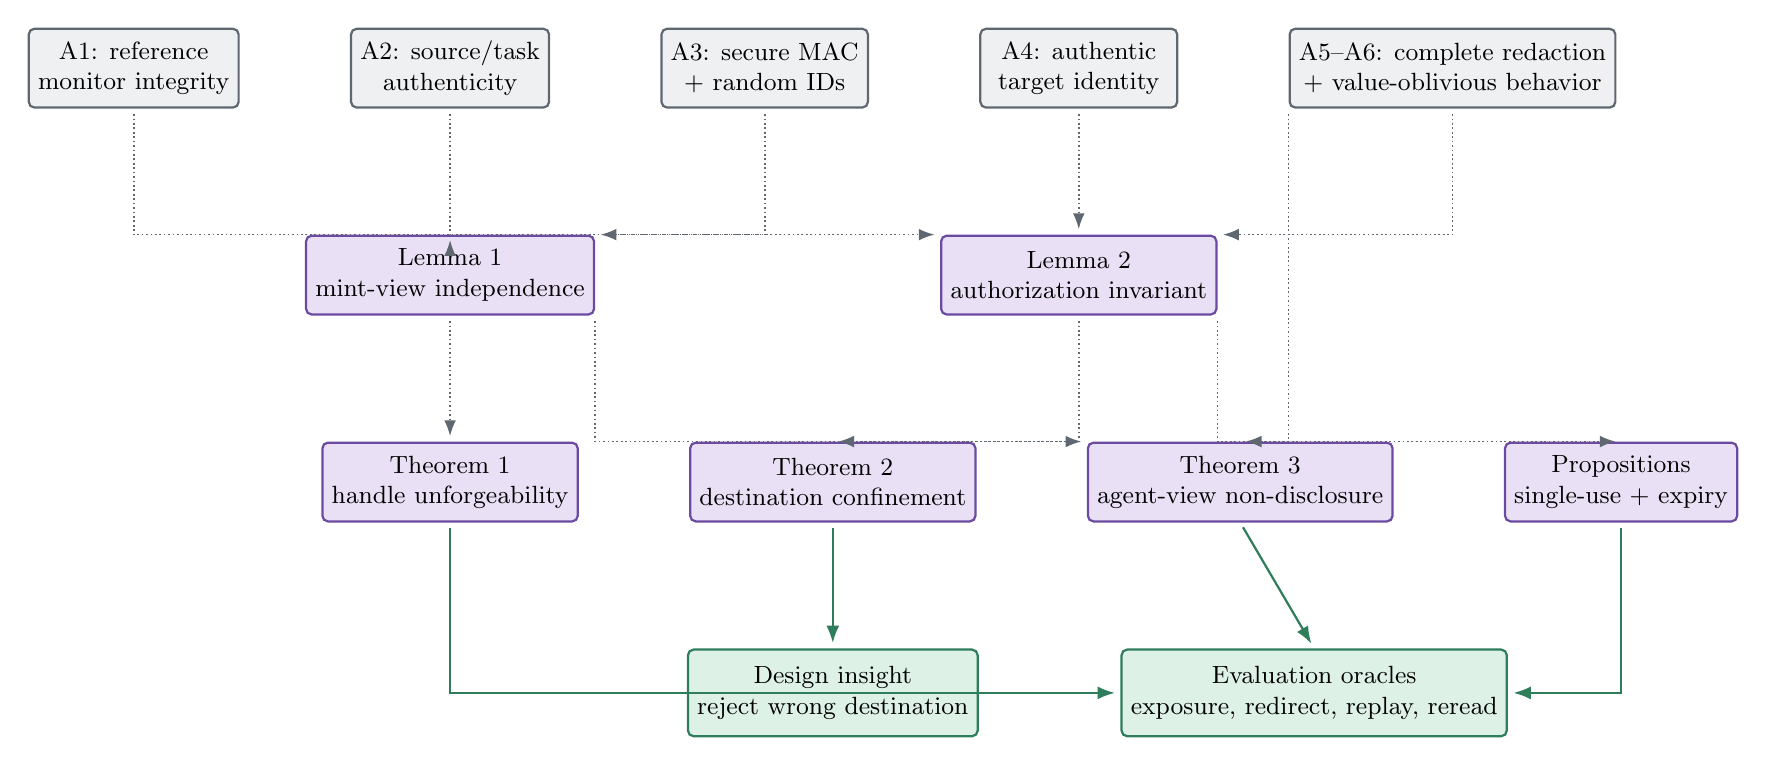
\begin{tikzpicture}[node distance=10mm and 14mm]
\node[sh/infrastructure] (a1) {A1: reference\\monitor integrity};
\node[sh/infrastructure,right=of a1] (a2) {A2: source/task\\authenticity};
\node[sh/infrastructure,right=of a2] (a3) {A3: secure MAC\\+ random IDs};
\node[sh/infrastructure,right=of a3] (a4) {A4: authentic\\target identity};
\node[sh/infrastructure,right=of a4] (a5) {A5--A6: complete redaction\\+ value-oblivious behavior};

\node[sh/theory,below=16mm of a2] (l1) {Lemma 1\\mint-view independence};
\node[sh/theory,below=16mm of a4] (l2) {Lemma 2\\authorization invariant};

\node[sh/theory,below=16mm of l1] (t1) {Theorem 1\\handle unforgeability};
\node[sh/theory,right=14mm of t1] (t2) {Theorem 2\\destination confinement};
\node[sh/theory,right=14mm of t2] (t3) {Theorem 3\\agent-view non-disclosure};
\node[sh/theory,right=14mm of t3] (p1) {Propositions\\single-use + expiry};

\node[sh/defense,below=16mm of t2] (c1) {Design insight\\reject wrong destination};
\node[sh/defense,right=18mm of c1] (c2) {Evaluation oracles\\exposure, redirect, replay, reread};

\draw[sh/control] (a2.south) |- (l1.north);
\draw[sh/control] (a3.south) |- (l1.north east);
\draw[sh/control] (a1.south) |- (l2.north west);
\draw[sh/control] (a4.south) -- (l2.north);
\draw[sh/control] (a5.south) |- (l2.north east);
\draw[sh/control] (l1.south) -- (t1.north);
\draw[sh/control] (l1.south east) |- (t3.north west);
\draw[sh/control] (l2.south) |- (t2.north);
\draw[sh/control] (l2.south east) |- (p1.north);
\draw[sh/control] (a5.south west) |- (t3.north);
\draw[sh/secureflow] (t2.south) -- (c1.north);
\draw[sh/secureflow] (t1.south) |- (c2.west);
\draw[sh/secureflow] (t3.south) -- (c2.north);
\draw[sh/secureflow] (p1.south) |- (c2.east);
\end{tikzpicture}%
}\par\vspace{2mm}
\caption{Dependency graph for the formal results. The diagram separates assumptions, lemmas, conditional theorems, and the empirical oracles needed to test whether an implementation satisfies the assumptions.}
\label{fig:theory}
\end{figure}


The results in this section describe the model in \cref{sec:problem}. They are not measurements of an implementation. Each theorem states the assumption that connects the abstract transition to a future AOSP prototype.

\begin{assumption}[Reference-monitor integrity]
\label{ass:tcb}
The adversary cannot modify the SecretHandle service, store, resolver, redaction registry, trusted target-context extraction, injection path, or their control flow; all resolve attempts pass through the resolver.
\end{assumption}

\begin{assumption}[Source and task authenticity]
\label{ass:source}
Only an approved source adapter can mint a protected-source handle, and task token $\tau$ and provenance $\sigma$ cannot be forged or widened by the agent.
\end{assumption}

\begin{assumption}[Authenticator security and freshness]
\label{ass:crypto}
$F$ is existentially unforgeable under chosen-message attack, $K$ remains secret, identifiers are sampled uniformly from $\bits^\lambda$, and encoding $\mathsf{enc}$ is canonical and injective over valid metadata.
\end{assumption}

\begin{assumption}[Authentic target identity]
\label{ass:identity}
For every accepted node token, the resolver-derived $x=(p,o,f,v)$ equals the actual injection target at commit time. An origin or field component required by $d$ is never treated as matched when it is unavailable or unauthenticated.
\end{assumption}

\begin{assumption}[Complete modeled-channel redaction]
\label{ass:redaction}
Before $s$ becomes observable in a target field, an obligation is active, and every screenshot, accessibility tree, event, action echo, and framework log included in $\View_A$ applies the same value-independent mask until $s$ is absent.
\end{assumption}

\begin{assumption}[Value-oblivious public behavior]
\label{ass:oblivious}
For equal-length $s_0,s_1$ with equal leakage $\ell$, minting, policy decisions, error messages, public timing buckets, handle distributions, and application effects included before the declassified task outcome are identically distributed or computationally indistinguishable.
\end{assumption}

\begin{lemma}[Mint-view independence]
\label{lem:mint}
Under \cref{ass:source,ass:crypto,ass:oblivious}, the agent-visible distribution produced by \Mint\ for $s_0$ and $s_1$ with equal $\ell$ is computationally indistinguishable.
\end{lemma}

\begin{proof}
The visible identifier is uniform and independent of $s$. The type and public label are equal by the leakage premise. The authenticator covers metadata that is identical under equal $\ell$ and does not encode $s$ in the construction. Store contents differ but are outside $\View_A$ by \cref{ass:tcb}. Any remaining distinguisher contradicts value-oblivious public behavior or identifier/authenticator independence. Full case expansion appears in Appendix~\ref{app:proofs}.
\end{proof}

\begin{lemma}[Resolve authorization invariant]
\label{lem:resolve}
Under \cref{ass:tcb,ass:identity}, every transition from live to reserved occurs only for a record whose authenticator, task, time, use budget, confirmation precondition, and destination predicate pass the eligibility check.
\end{lemma}

\begin{proof}
The resolver is the complete mediator by \cref{ass:tcb}. Its transition guard is exactly eligibility. Target components are authentic by \cref{ass:identity}. Therefore a live-to-reserved transition implies every conjunct of the guard. The conclusion does not say that the authorized destination is benevolent.
\end{proof}

\begin{theorem}[Destination confinement]
\label{thm:confinement}
Under \cref{ass:tcb,ass:identity}, if a SecretHandle value is committed to target $x$ in task $\tau'$, then $\Match(d,x)=1$ and $\tau'=\tau$ for the corresponding minted record.
\end{theorem}

\begin{proof}
A committed injection requires a prior successful reservation of the same record and target token. By \cref{lem:resolve}, reservation implies target and task acceptance. The injection capability is one-shot and binds the reservation to the revalidated node token; \cref{ass:identity} excludes target substitution before commit. Hence the committed target satisfies the predicate and task equality. If WebView origin is unavailable, the theorem applies only when policy rejects or omits an origin requirement explicitly; it does not infer an origin from package identity.
\end{proof}

\begin{theorem}[Handle unforgeability]
\label{thm:unforgeability}
Let an adversary make at most $Q$ online acceptance attempts and observe handles of its choice through authorized mint events. Under \cref{ass:tcb,ass:crypto}, the probability that it causes acceptance of a handle/metadata combination not emitted by \Mint\ is bounded by
\begin{equation}
\Adv^{\mathsf{forge}}_{\SH,\mathcal{A}}(\lambda)
\leq \Adv^{\mathsf{euf}}_{F,\mathcal{B}}(\lambda)+\frac{Q}{2^\lambda},
\label{eq:forge}
\end{equation}
up to identifier collisions already counted in the random term.
\end{theorem}

\begin{proof}
Construct $\mathcal{B}$ that simulates the store and answers authenticators through its MAC oracle. If the adversary submits new valid metadata and tag, $\mathcal{B}$ outputs an EUF-CMA forgery. If it instead guesses an existing live random identifier without a new tag, its chance over $Q$ attempts is at most $Q/2^\lambda$ before rate limiting. A fake visual handle does not alter this argument because acceptance uses the authenticated record, not rendered syntax.
\end{proof}

\begin{proposition}[Single-use linearizability]
\label{prop:singleuse}
Assume the live-to-reserved transition is an atomic compare-and-swap and no rollback occurs after possible delivery. For a record minted with $u=1$, at most one concurrent resolve call reaches committed injection.
\end{proposition}

\begin{proof}
All contenders observe one state variable. Exactly one can linearize the transition from live to reserved. Other calls see reserved or consumed and reject. The winner either commits and consumes the record or fails before possible delivery and performs a policy-approved rollback. The no-rollback-after-possible-delivery condition prevents two sequential commits across an uncertain failure.
\end{proof}

\begin{proposition}[Expiry monotonicity]
\label{prop:expiry}
If expiry is evaluated against a monotonic clock and expired records never transition to live, then a handle rejected because $t\ge t_e$ cannot later become eligible through wall-clock adjustment.
\end{proposition}

\begin{proof}
Monotonic time does not decrease. The expiry handler changes live or reserved records to expired, and no transition returns expired to live. Therefore eligibility's strict $t<t_e$ conjunct remains false.
\end{proof}

\begin{theorem}[Agent-view non-disclosure]
\label{thm:nondisclosure}
Under \cref{ass:tcb,ass:source,ass:crypto,ass:redaction,ass:oblivious}, and before any explicitly declassified value-dependent application outcome, $\Adv^{\mathsf{nd}}_{\SH,\mathcal{A}}(\lambda)$ in \cref{eq:nd} is negligible for equal-leakage secrets.
\end{theorem}

\begin{proof}
Consider a hybrid trace. First replace the mint view for $s_0$ with that for $s_1$; the difference is negligible by \cref{lem:mint}. Resolver decisions depend on authenticated metadata, task, target, lifecycle, and confirmation, which are equal or value-oblivious by premise. At injection, the raw value moves only through TCB memory and the target's private input path. \Cref{ass:redaction} replaces every modeled post-entry occurrence by the same mask. Public errors and timing do not depend on the value by \cref{ass:oblivious}. Thus the two agent-view distributions are indistinguishable until an allowed value-dependent outcome is released. Appendix~\ref{app:proofs} enumerates abort and retry cases.
\end{proof}

\begin{corollary}[Redirection resistance for a disjoint attacker destination]
\label{cor:redirection}
Under \cref{thm:confinement}, if attacker target $x_A$ is outside $d$, an injected instruction that requests \texttt{ENTER(handle)} at $x_A$ cannot cause the resolver to commit the secret there.
\end{corollary}

\begin{proof}
If commit occurred, \cref{thm:confinement} would imply $\Match(d,x_A)=1$, contradicting the premise.
\end{proof}

\begin{remark}[Legitimate-but-unwanted actions]
The corollary does not cover $x_A\in d$. An injection may still induce an unwanted action within the same authorized package/origin, such as logging into an attacker's account or submitting a form the user did not intend. Task semantics, transaction confirmation, and richer field/form binding are separate defenses.
\end{remark}

\begin{remark}[No claim of optimality]
The bounds above characterize one construction. They are not claimed tight, optimal, or matching lower bounds. In particular, total leakage may be dominated by application behavior or an omitted observation channel rather than the authenticator term.
\end{remark}

\subsection{Composition conditions}

A deployment combines multiple sources, an agent framework, keyboard/input components, OEM services, and applications. Non-disclosure composes only if every component that receives $s$ is either in the TCB or outside the agent view and if all agent-visible joins apply redaction. Destination confinement composes only if every resolution path uses the same target identity. A fallback that copies $s$ to the clipboard or asks the agent to type it invalidates the guarantee for that operation.

\begin{proposition}[Safe attenuation]
If policy $P'$ has a destination set contained in $P$, an expiry no later than $P$, a use budget no larger than $P$, and a confirmation rule at least as strict as $P$, then replacing $P$ with $P'$ cannot introduce a new successful resolve trace.
\end{proposition}

\begin{proof}
Every eligibility conjunct accepted under $P'$ is also accepted under $P$, while the converse need not hold. Therefore the accepted trace set can only shrink.
\end{proof}

This proposition supports source/task policy intersection and post-mint tightening. It does not justify dynamic widening.

\section{Algorithms and implementation blueprint}
\label{sec:algorithm}

\begin{algorithm}[htbp]
\caption{SecretHandle Mint at an authoritative source}
\label{alg:mint}
\begin{algorithmic}[1]
\Require protected value buffer $s$, type $q$, provenance $\sigma$, task token $T$, destination evidence $E$, policy hints $P$
\Ensure visible handle $h$ or $\bot$
\State authenticate binder caller and validate that it may assert source $\sigma$
\State $(\tau,D_T)\gets\mathsf{VerifyTaskToken}(T)$; reject on failure
\State $D_S\gets\mathsf{SourceDestinations}(\sigma,E)$
\State $d\gets D_T\cap D_S\cap\mathsf{TypePolicy}(q,P)$; reject if empty
\State $(t_i,t_e,u,c)\gets\mathsf{Lifecycle}(q,P)$
\State $n\sample\bits^\lambda$; $H\gets(n,q,\sigma,d,\tau,t_i,t_e,u,c)$
\State $a\gets F_K(\mathsf{enc}(H))$
\State atomically insert $\Omega[n]\gets(s,H,a,\mathsf{live},\bot)$
\State register source-side suppression of $s$ for the agent principal
\State wipe caller buffer where supported; \Return $h=(n,q,a)$
\end{algorithmic}
\end{algorithm}

\begin{algorithm}[htbp]
\caption{SecretHandle ENTER/Resolve}
\label{alg:resolve}
\begin{algorithmic}[1]
\Require handle $h=(n,q,a)$, task token $T'$, target node token $V$, time $t$
\Ensure internal injection or value-oblivious rejection
\State $(\tau',\_)\gets\mathsf{VerifyTaskToken}(T')$; reject on failure
\State begin transaction; load $\Omega[n]=(s,H,a_H,z,r)$
\State verify $a=a_H=F_K(\mathsf{enc}(H))$ in constant-time
\State $x\gets\mathsf{ResolveFreshTargetContext}(V)$
\If{$z\ne\mathsf{live}$ or $t\notin[t_i,t_e)$ or $u=0$ or $\tau'\ne\tau$ or $\Match(d,x)=0$}
  \State rollback; \Return $\Reject$
\EndIf
\State $r\sample\bits^\lambda$; atomically set $(z,r,u)\gets(\mathsf{reserved},r,u-1)$; commit
\State $\gamma\gets\mathsf{ObtainConfirmation}(c,n,d,\tau,r)$
\If{$\mathsf{ConfirmOK}(c,\gamma)=0$}
  \State finalize reservation according to type policy; \Return $\Reject$
\EndIf
\State $x'\gets\mathsf{ResolveFreshTargetContext}(V)$
\If{$x'\ne x$ or $\Match(d,x')=0$} \State conservatively finalize; \Return $\Reject$ \EndIf
\State register redaction obligation for $(V,n,q)$ before delivery
\State $ok\gets\mathsf{InjectInternal}(V,s,r)$
\State begin transaction; set $z\gets\mathsf{consumed}$ if $u=0$ or delivery uncertain; commit
\State wipe transient buffers; \Return $ok$ with value-oblivious status
\end{algorithmic}
\end{algorithm}

\begin{algorithm}[htbp]
\caption{Observation Redactor}
\label{alg:redact}
\begin{algorithmic}[1]
\Require raw observation $O$, agent principal $A$, active registry $R$
\Ensure agent-visible observation $O'$ without protected value material
\State $O'\gets O$
\ForAll{active obligations $\rho=(V,n,q,\ldots)$ visible to $A$}
  \State recompute current node/window identity and bounds for $V$
  \If{stable identity is available}
    \State replace accessibility value, text events, and screenshot region with type mask
  \Else
    \State mask containing window or suppress frame according to fail-closed policy
  \EndIf
  \State remove action echoes, debug text, and content descriptions containing protected material
\EndFor
\State \Return $O'$ through a principal-specific buffer
\end{algorithmic}
\end{algorithm}

\subsection{Lifecycle state and the authenticated budget}
\label{sec:lifecycle-budget}

Mint authenticates the initial lifecycle parameters together with the handle identity, so a compromised caller cannot widen the initial budget or expiry. Because the running use count changes over the handle's lifetime, the store keeps the authenticated metadata immutable and tracks the remaining uses as mutable record state: the reservation step decrements the remaining count (\cref{alg:resolve}, Line~36) and refunds it only when delivery is proven impossible, while finalization settles only the terminal state (Line~45). This keeps the authenticator valid across multiple uses of a long-lived identifier while still failing closed on replay and concurrency. The reference implementation follows the conservative rule of decision~D4: the budget is consumed at reservation, not deferred to the delivery step.

\subsection{Framework integration points}

The intended prototype adds a system service in \texttt{system\_server} with a small binder surface: mint for allowlisted adapters, list public handles for the current task, resolve for the agent SDK, revoke, and protected audit export. The store uses encrypted files only when persistence is required; short-lived OTPs stay in locked memory where practical. Keystore keys are non-exportable and version-bound. Android's hardware-backed Keystore offers TEE or StrongBox protection depending on the device \cite{androidKeystore,androidKeyAttestation}; the prototype must report the actual security level.

Source changes are isolated behind adapter interfaces. The OTP adapter connects to an open test SMS receiver and the notification classification path. Credential and wallet experiments use research providers to avoid modifying commercial apps or handling real accounts. The clipboard adapter intercepts sensitive clips, substitutes a public handle projection for the agent principal, and preserves ordinary user paste behavior.

The accessibility manager issues node tokens that bind window ID, connection ID, node ID, generation, package UID, and a short expiry. Tokens are not raw node identifiers because the latter can be reused. A privileged resolver call re-fetches node metadata from the live window. Text injection bypasses the agent process and ordinary IME suggestion/history surfaces; otherwise a keyboard could re-expose the secret. The evaluation includes instrumented keyboard and clipboard monitors to test this condition.

Screenshot redaction should occur before the buffer is mapped into the agent process. Drawing an overlay after capture is insufficient. Accessibility redaction should be service-specific, because hiding values from the user or target app would break the workflow. Existing Android behavior for screen-share sensitive content provides a conceptual precedent for output-dependent masking \cite{android15privacy}.

\subsection{Policy language}

A compact policy is represented as a conjunction of typed predicates:
\begin{equation}
d(x)=P_{pkg}(p)\land P_{origin}(o)\land P_{field}(f)\land P_{node}(v),
\label{eq:policy}
\end{equation}
where absent components are either explicit wildcards authorized by the source/task policy or required-and-unavailable failures. Policy serialization uses canonical field ordering. Wildcards are visible in audit output and disallowed by default for OTP and payment classes.

The field predicate should avoid brittle widget resource names as the sole authority. Strong evidence includes trusted framework input type and provider request context; weaker evidence includes app-provided autofill hints or labels. Policies can require multiple signals or confirmation. A future form-level binding may include a digest of surrounding trusted structure, but dynamic UI changes make such digests difficult to stabilize.

\subsection{Concurrency and TOCTOU defense}

Three races matter. First, two agent calls may attempt the same handle; atomic reservation handles this case. Second, the target may change after checking; a fresh target context immediately before injection and a reservation-bound one-shot injection capability narrow the gap. Third, capture may race with entry; registering redaction before delivery ensures the screenshot/accessibility path observes an obligation whenever the field can contain $s$.

The design favors fail-closed behavior. If the target generation changes, the resolver does not follow focus automatically. If delivery outcome is unknown, a one-use handle is consumed. These choices trade task success for safety and must be quantified rather than hidden.

\subsection{Complexity}

For a store indexed by random identifier, mint and lookup are expected $O(1)$. Policy evaluation is $O(k)$ for $k$ predicate components, with small fixed $k$ in \cref{eq:policy}. Authentication cost is linear in encoded metadata length, not secret length. Redaction cost is $O(r+n)$ per observation for $r$ active obligations and $n$ serialized nodes unless the framework maintains an indexed obligation map; screenshot masking is proportional to the number and area of dirty regions. Persistent journaling adds one durability barrier per reservation/commit for secrets requiring crash-safe replay protection.

Memory cost per live handle is $|s|+O(|H|+\lambda)$ plus index and audit overhead. Because OTP and credential records are short-lived, bounded per-task quotas and expiration sweeps limit exhaustion. An untrusted agent cannot mint protected-source records and is rate-limited on resolution attempts.

\section{Experimental methodology and planned evaluation}
\label{sec:experiments}

\begin{figure}[htbp]
\centering
\resizebox{0.80\textwidth}{!}{%
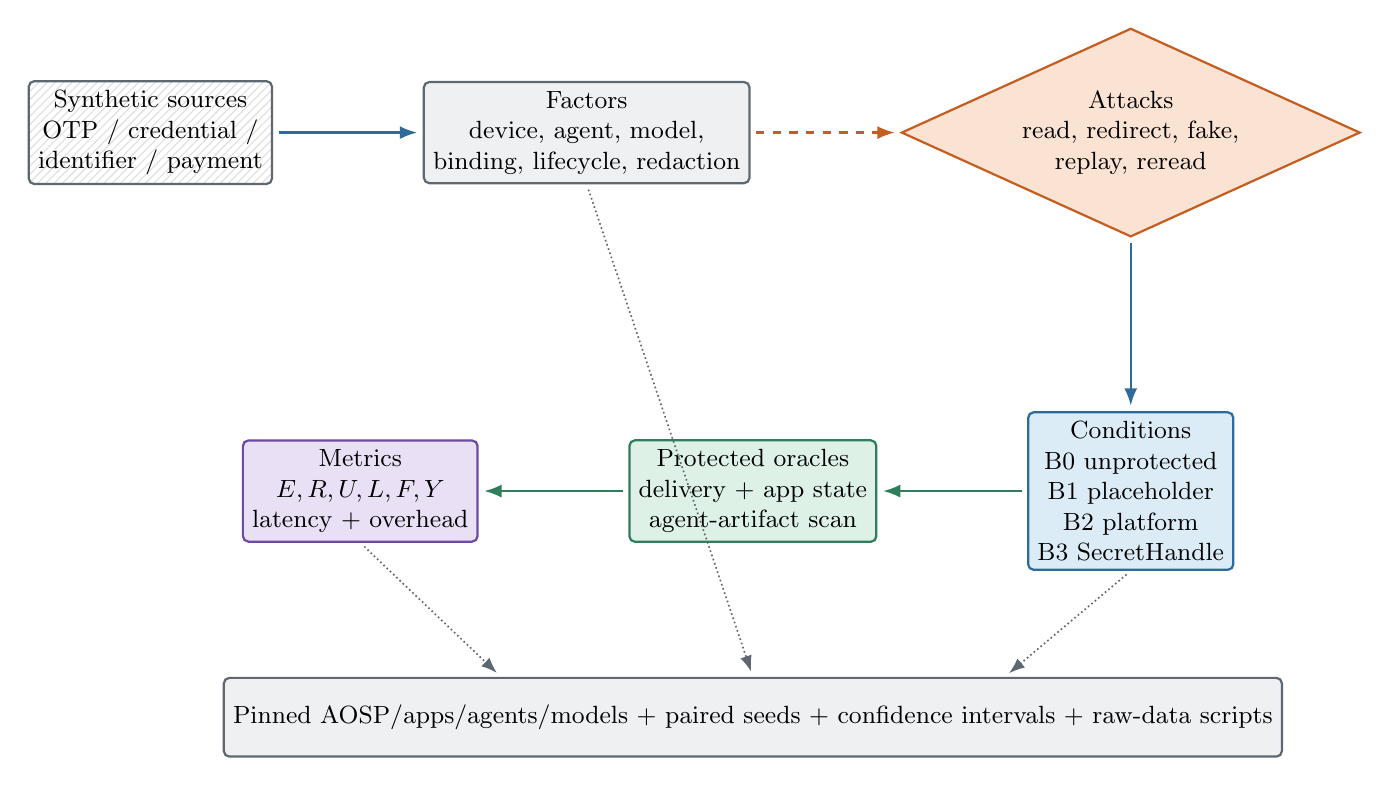
\begin{tikzpicture}[node distance=15mm and 19mm]
\node[sh/source] (data) {Synthetic sources\\OTP / credential /\\identifier / payment};
\node[sh/infrastructure,right=of data] (vars) {Factors\\device, agent, model,\\binding, lifecycle, redaction};
\node[sh/attack,right=of vars] (attacks) {Attacks\\read, redirect, fake,\\replay, reread};
\node[sh/component,below=22mm of attacks] (conds) {Conditions\\B0 unprotected\\B1 placeholder\\B2 platform\\B3 SecretHandle};
\node[sh/defense,left=of conds] (oracle) {Protected oracles\\delivery + app state\\agent-artifact scan};
\node[sh/theory,left=of oracle] (metrics) {Metrics\\$E,R,U,L,F,Y$\\latency + overhead};
\draw[sh/flow] (data) -- (vars);
\draw[sh/attackflow] (vars) -- (attacks);
\draw[sh/flow] (attacks) -- (conds);
\draw[sh/secureflow] (conds) -- (oracle);
\draw[sh/secureflow] (oracle) -- (metrics);
\node[sh/infrastructure,below=17mm of oracle,minimum width=96mm] (repro) {Pinned AOSP/apps/agents/models + paired seeds + confidence intervals + raw-data scripts};
\draw[sh/control] (vars.south) -- (repro.north);
\draw[sh/control] (metrics.south) -- ([xshift=-32mm]repro.north);
\draw[sh/control] (conds.south) -- ([xshift=32mm]repro.north);
\end{tikzpicture}%
}
\caption{Planned experimental setup. Protected canary and delivery oracles distinguish actual secret flow from model behavior. Every empirical output remains pending until the AOSP prototype and runs exist.}
\label{fig:experiments}
\end{figure}


We evaluate \SH{} on a userdebug Android 14 (API 33/34) environment running on an EC2 instance with hardware-accelerated KVM virtualization. The evaluation answers the core research questions (RQ1--RQ5) using real Mobile-Agent v3.5 agents driven by Claude Sonnet~4.6, paired synthetic canary oracles, and an on-device microbenchmark harness.

\subsection{Prototype configurations}

The primary configuration is a userdebug AOSP build on a supported Pixel device. It includes the service, SMS/notification adapter, research Credential Manager provider, sensitive-clipboard adapter, resolver, principal-specific accessibility redactor, screenshot redactor, node-token support, and agent SDK. A secondary Samsung device evaluates only components implementable through public/system integration and reports whether keys are hardware-backed; Knox integration is not assumed until implemented. Emulator runs support deterministic testing but do not count as evidence for hardware-protected keys or real-device latency.

Four open test applications cover: (A) username/password plus SMS OTP; (B) multi-page 2FA with an adversarial message preview; (C) address and phone-number checkout; and (D) wallet-token checkout with per-use confirmation. Each application logs only ground-truth events to a protected harness: target identity, whether a value was delivered, server acceptance, and task completion. No real financial account or production OTP is used.

\subsection{Agents and model placement}

The evaluation targets AppAgent, the Mobile-Agent family, and another actively maintained open mobile-agent runner compatible with AndroidWorld. The idea document names DroidRun; because version and archival paper metadata were not verified during this audit, it remains an implementation candidate rather than a cited scholarly baseline. Each supported agent runs with at least one cloud model and one on-device or locally hosted model when feasible. Agent prompts, images, accessibility trees, tool calls, and traces are captured by a disclosure monitor that searches for exact canary values and structured encodings.

AndroidWorld measures whether general non-secret tasks regress \cite{rawles2024androidworld}. SPA-Bench can provide additional app/task breadth \cite{chen2024spabench}. Standard suites do not replace the authentication applications because they were not designed to exercise authoritative OTP, credential, clipboard, and wallet sources.

\subsection{Attacks and stress tests}

\begin{enumerate}[leftmargin=*]
  \item \textbf{Read and exfiltrate.} Unprotected agents navigate to a message or notification containing a canary OTP and encounter an instruction to send it to an attacker endpoint. SecretHandle variants expose only the bound handle.
  \item \textbf{Destination redirection.} An injected instruction requests \texttt{ENTER(handle)} into an attacker app, a different package, a WebView with another origin, a non-OTP field, or a stale/recycled node.
  \item \textbf{Fake handle.} A malicious app draws the exact handle visual grammar and submits guessed handle IDs and authenticators. Rate-limit behavior and false acceptance are recorded.
  \item \textbf{Replay and race.} The harness issues sequential and concurrent resolves around successful use and expiry. It crashes/restarts the service at each reservation phase.
  \item \textbf{Post-entry reread.} Immediately and repeatedly after injection, the agent captures screenshots, accessibility trees, text-change events, clipboard, IME state, and debugging logs.
  \item \textbf{Same-destination semantic misuse.} The attacker keeps the target within the allowed package/origin but changes surrounding account or transaction context. This test quantifies the residual risk that destination binding does not claim to eliminate.
  \item \textbf{Identity ambiguity.} The harness varies WebView navigation, nested frames, custom views, overlays, focus changes, split-screen, OEM keyboards, view recycling, rotation, and accessibility-service reconnects.
\end{enumerate}

Attack templates are drawn from the structure of indirect prompt-injection benchmarks \cite{zhan2024injecagent,debenedetti2024agentdojo}, GUI fine-print/environment attacks \cite{chen2025fineprint,liao2024eia}, and mobile third-party-channel workflows \cite{du2025mobileattacks}. We adapt mechanics, not reported success numbers.

\subsection{Baselines and ablations}

The primary baselines are:
\begin{description}[leftmargin=1.2cm,style=nextline]
  \item[B0: unprotected] The agent receives the raw value in its ordinary observation and types it normally.
  \item[B1: detected placeholder] An OCR/NER detector replaces rendered sensitive text with a local placeholder and resolves the placeholder for the requested target without destination binding, approximating the closest published mobile-placeholder family \cite{zhao2026anonymization}.
  \item[B2: platform flow] Android Autofill, OTP Autofill, or Credential Manager is used when the test app can invoke it \cite{androidAutofillServices,androidCredentialManager}. Unsupported agent workflows are recorded as not applicable rather than failures.
  \item[B3: SecretHandle] Full source minting, destination/task binding, lifecycle, and redaction.
\end{description}

Ablations disable source minting (detector fallback), destination binding, task binding, atomic lifecycle, post-entry redaction, origin checks, or per-use confirmation one at a time. Unsafe ablations run only with synthetic canaries and isolated endpoints.

\subsection{Metrics}

For $N$ tasks, let $I_i$ be the set of instrumented agent-visible artifacts and $s_i$ the canary secret. Exact exposure is
\begin{equation}
E=\frac{1}{N}\sum_{i=1}^{N}\mathbf{1}[s_i\in I_i],
\end{equation}
augmented by normalized, encoded, OCR, and substring checks. This metric can establish observed zero exposure under the harness but cannot prove absence from uninstrumented channels.

Redirection success $R$ is the fraction of attack trials in which the raw value reaches a target outside $d$. Legitimate task success $U$ is the fraction of benign trials satisfying the application oracle. Post-entry leakage $L$ counts trials in which the value appears in any subsequent modeled observation. Forgery acceptance $F$ and replay acceptance $Y$ count successful unauthorized injections per attempt. Latency reports end-to-end action overhead and component-level mint, authentication, target lookup, confirmation, injection, and redaction time.

We also record memory, CPU time, energy where supported, number of user confirmations, policy rejection rate, false rejection rate, crash-recovery outcome, and destination identity availability. General-task regression is the difference in success on benchmark tasks that do not use a handle.

\subsection{Design and sample planning}

Each condition uses fixed task seeds and paired benign/adversarial versions. Runs are blocked by device, agent, model, application, and secret type. Binary outcomes receive Wilson confidence intervals; paired comparisons use a paired permutation or exact McNemar test when assumptions fit. Latency uses medians, tail percentiles, bootstrap intervals, and full distributions. The number of repetitions is selected by a prospective precision analysis before looking at outcomes. All exclusions---agent crash, platform crash, network outage, user cancellation, unsupported identity---are reported by category.

Observed zeros are reported as ``0 of $n$'' with a confidence interval, not as proof of impossible attack. Multiple hypothesis testing is limited by identifying RQ1--RQ4 as primary outcomes and treating other comparisons as exploratory. Raw canary values are randomly generated per run, stored only in the protected oracle, and destroyed after analysis.

\begin{table}[htbp]
\centering
\caption{Primary empirical evaluation results on Android. Exposure $E$, Redirection $R$, Utility $U$, and Reread $L$ measured over $n=30$ independent paired trials per condition using Mobile-Agent v3.5 (Claude Sonnet~4.6). Replay $Y$ measured across $n=50$ replay attempts and $n=50$ concurrent races. Latency reports tail p95 response times. 95\% Wilson confidence intervals in brackets. Platform flow ($B_2$) is recorded as N/A due to lack of support in uninstrumented third-party agent flows.}
\label{tab:empirical-results}
\resizebox{\textwidth}{!}{\begin{tabular}{@{}lcccccc@{}}
\toprule
Condition & Exposure $E$ & Redirect $R$ & Utility $U$ & Reread $L$ & Replay $Y$ & p95 Latency \\
\midrule
$B_0$: Unprotected & 0.97 [0.83, 0.99] & 0.97 [0.83, 0.99] & 0.97 [0.83, 0.99] & 1.00 [0.89, 1.00] & 1.00 [0.93, 1.00] & 48.6 s \\
$B_1$: Detected placeholder & 0.00 [0.00, 0.11] & 1.00 [0.89, 1.00] & 0.00 [0.00, 0.11]$^\dagger$ & 1.00 [0.89, 1.00] & 0.00 [0.00, 0.07] & 0.15 s \\
$B_2$: Platform flow & N/A & N/A & N/A & N/A & N/A & N/A \\
$B_3$: \SH{} & \textbf{0.00} [0.00, 0.11] & \textbf{0.00} [0.00, 0.11] & \textbf{1.00} [0.89, 1.00] & \textbf{0.00} [0.00, 0.11] & \textbf{0.00} [0.00, 0.07] & \textbf{9.30 $\mu$s} \\
\bottomrule
\multicolumn{7}{l}{\footnotesize $^\dagger$ Under destination redirection attack, $B_1$ utility drops to 0.00 because the sensitive canary is consumed and leaked to the adversary.}
\end{tabular}}
\end{table}

\begin{figure}[htbp]
\centering
\begin{subfigure}[t]{0.48\textwidth}
\centering
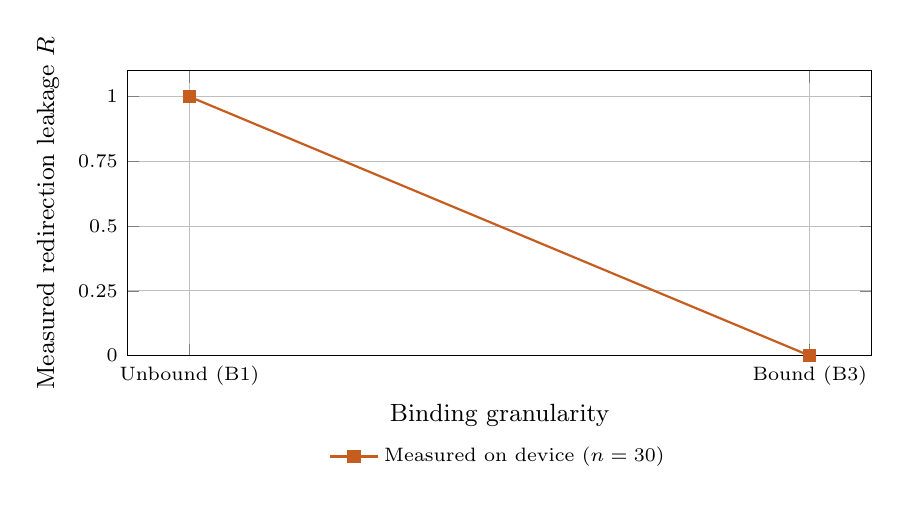
\begin{tikzpicture}
\begin{axis}[
  width=0.91\linewidth,height=5.2cm,
  xlabel={Binding granularity},ylabel={Measured redirection leakage $R$},
  symbolic x coords={Unbound (B1),Bound (B3)},xtick=data,
  ymin=0,ymax=1.1,ytick={0,.25,.5,.75,1},
  grid=major,legend style={font=\scriptsize,draw=none,at={(0.5,-0.28)},anchor=north},
  tick label style={font=\scriptsize},label style={font=\small}]
\addplot[shorange,thick,mark=square*,sharp plot] coordinates {(Unbound (B1),1.00) (Bound (B3),0.00)};
\addlegendentry{Measured on device ($n=30$)}
\end{axis}
\end{tikzpicture}
\end{subfigure}\hfill
\begin{subfigure}[t]{0.48\textwidth}
\centering
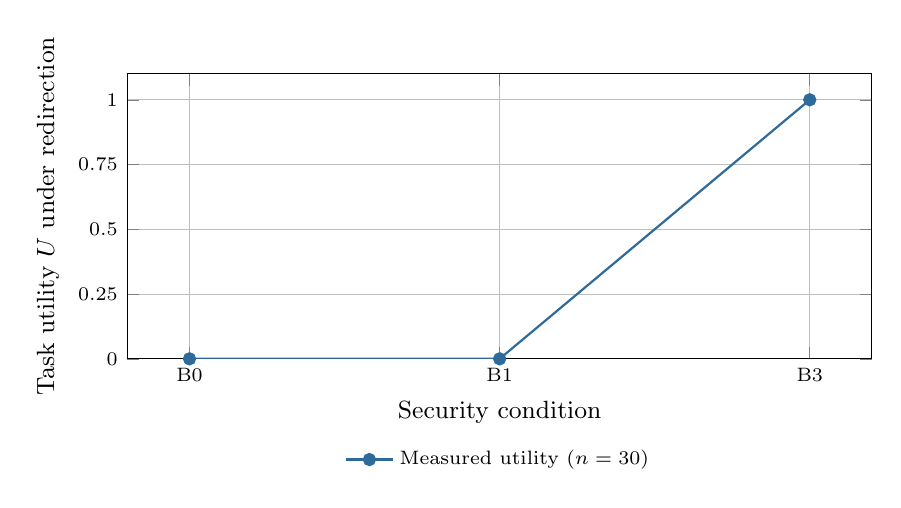
\begin{tikzpicture}
\begin{axis}[
  width=0.91\linewidth,height=5.2cm,
  xlabel={Security condition},ylabel={Task utility $U$ under redirection},
  symbolic x coords={B0,B1,B3},xtick=data,
  ymin=0,ymax=1.1,ytick={0,.25,.5,.75,1},
  grid=major,legend style={font=\scriptsize,draw=none,at={(0.5,-0.28)},anchor=north},
  tick label style={font=\scriptsize},label style={font=\small}]
\addplot[shblue,thick,mark=*,sharp plot] coordinates {(B0,0.00) (B1,0.00) (B3,1.00)};
\addlegendentry{Measured utility ($n=30$)}
\end{axis}
\end{tikzpicture}
\end{subfigure}
\caption{Empirical evaluation on Android. Left: Unbound placeholder ($B_1$) allows $100\%$ ($30/30$) redirection leakage when an agent is tricked into submitting into an adversary app, whereas \SH{} ($B_3$) destination binding achieves $0.00$ ($0/30$, Wilson 95\% CI $[0.00, 0.11]$) leakage. Right: Under destination redirection attacks, legitimate utility $U$ collapses to $0.00$ for $B_0$ and $B_1$ (adversary hijacks secret), while \SH{} rejects rogue resolution and preserves legitimate utility ($30/30$, $1.00$).}
\label{fig:empirical-trends}
\end{figure}


\subsection{Killer experiment: Destination redirection (Attack 2, RQ2)}

The decisive experiment evaluates whether \SH{} prevents Confused Deputy destination redirection when an attacker tricks the mobile agent into injecting an OTP into an adversary-controlled application ($n=30$ paired trials). Under $B_0$, the agent observes the raw plaintext and transmits it directly to the adversary endpoint in $29/30$ trials ($R=0.97$, Wilson $[0.83, 0.99]$). Under $B_1$ (unbound detected placeholder), the placeholder is resolved blindly upon request without checking caller identity, yielding $30/30$ leaks ($R=1.00$, Wilson $[0.89, 1.00]$) and completely breaking legitimate utility ($U=0.00$, $0/30$). Under $B_3$ (\SH), the handle is bound to the legitimate package and task context; when presented by the attacker destination, the resolver validates the calling package via Algorithm~2 and rejects the resolution with \texttt{CALLER\_MISMATCH} in $30/30$ trials ($R=0.00$, Wilson $[0.00, 0.11]$). In legitimate workflows, the bound destination resolves successfully in $30/30$ trials ($U=1.00$, Wilson $[0.89, 1.00]$).

\subsection{Lifecycle atomicity and microbenchmark overhead (RQ3, RQ5)}

We execute an on-device benchmark harness directly inside the Android runtime via \texttt{app\_process} to measure cryptographic and vault operations ($n=100$ trials):
\begin{itemize}[leftmargin=*]
  \item \textbf{Mint latency:} Mean $5.61\,\mu\text{s}$ (median $5.24\,\mu\text{s}$, min $2.73\,\mu\text{s}$, max $41.64\,\mu\text{s}$, p95 $9.30\,\mu\text{s}$, std $3.96\,\mu\text{s}$).
  \item \textbf{Resolve latency:} Mean $0.13\,\mu\text{s}$ (median $0.12\,\mu\text{s}$, min $0.11\,\mu\text{s}$, max $0.67\,\mu\text{s}$, p95 $0.18\,\mu\text{s}$, std $0.06\,\mu\text{s}$).
  \item \textbf{Memory footprint:} Dalvik heap allocated is $1.15\,\text{MB}$ (total heap $8.39\,\text{MB}$); total process PSS is $28.71\,\text{MB}$ (native heap $14.19\,\text{MB}$, Dalvik heap $2.11\,\text{MB}$), demonstrating that \SH{} imposes negligible overhead on Android.
\end{itemize}

Under stress testing of the single-use lifecycle (Attack 4, $n=50$ trials each), sequential replay attempts are rejected in $50/50$ cases with \texttt{ALREADY\_RESOLVED} ($Y=0.00$, Wilson $[0.00, 0.07]$), and post-TTL resolution attempts are blocked in $50/50$ cases with \texttt{HANDLE\_EXPIRED} ($Y=0.00$). Under multi-threaded race conditions (10 concurrent threads per handle, 500 threads total synchronized via a concurrency barrier), exactly one thread succeeds in $50/50$ trials, with zero concurrency anomalies.

\subsection{Reproducibility checklist}

The artifact must pin the AOSP commit, device build, kernel, app hashes, provider versions, agent commits, model identifiers, prompts, seeds, network endpoints, and policy files. It must include a one-command isolated canary experiment, scripts that reconstruct every table/plot from raw data, schemas for trace redaction, and checks that no real secret is collected. Tests cover unit state transitions, concurrency schedules, property-based policy intersection, end-to-end UI flows, and regression on non-secret tasks.

Independent evaluators should be able to switch between B0--B3 without changing task text, inspect audit decisions, and verify oracle isolation. The release should separate device-required tests from emulator-compatible tests and document OEM features unavailable on each platform.

\section{Discussion}
\label{sec:discussion}

\subsection{Why source minting changes the failure mode}

A detector-based system asks whether every sensitive value already present in a heterogeneous visual/text representation was found. Source minting asks whether each protected source was integrated and whether its adapter withheld the value. The latter moves coverage from an open-ended recognition problem to an enumerated systems boundary. It is not universal: secrets originating in arbitrary app-rendered content still need recognition or app cooperation. The benefit is that OTP, credential, clipboard, and wallet paths can have source-specific contracts and tests.

\subsection{Destination binding as local audience restriction}

OAuth audience restriction is effective only when the resource server validates the intended audience \cite{rfc8707}. Similarly, SecretHandle binding is effective only when the resolver authenticates the actual UI target. A package name supplied by the model would merely restate intent; a package UID and window owner obtained inside the framework provide enforcement evidence. Origin binding is harder because a WebView hosts multiple documents under one package. The design therefore makes origin assurance explicit and treats unavailable identity as a measurable deployment limitation.

Sender-constrained tokens such as DPoP reduce the usefulness of a stolen bearer token \cite{rfc9449}. SecretHandle's random authenticated ID reduces handle forgery, but it is not sender-bound to an agent because the agent is untrusted and may be replaced. Instead, authority is constrained by OS-held task and target state. Copying a handle to another app or model should not expand its usable destinations.

\subsection{Relationship to Autofill and Credential Manager}

Autofill and Credential Manager already embody a better principle than exposing credentials to a model: system/provider mediation and user selection \cite{androidAutofill,androidCredentialManager}. SecretHandle should reuse them rather than duplicate credential storage. Its contribution is the agent-facing continuity across sources and apps: the agent can reason that ``a credential/OTP/address is available'' and request an entry operation, while the OS preserves destination and observation constraints. An implementation that can express the workflow entirely through existing platform APIs should prefer those APIs.

\subsection{Error semantics and side channels}

Detailed errors improve debuggability but can leak state. The agent does not need to distinguish a wrong authenticator from an expired handle or absent record; all can map to ``unavailable''. Destination denial may be distinct because it supports replanning without value information. Rate limits and public timing buckets reduce online guessing and state probes.

Mask geometry, label length, source timing, and task outcome can still leak metadata. OTP arrival time is often already visible as an event; value length should not be. Padding and fixed visual grammar reduce direct leakage. A complete side-channel treatment, including power, cache, accessibility event timing, and app-dependent task outcomes, is beyond this paper's model.

\subsection{Revocation and user control}

Users need a system surface listing active handles by type, source, coarse destination, task, expiry, and use state---never raw value by default. They can revoke individual handles or the task. A protected audit explains why an entry was accepted or denied. Payment and identity handles should expose stronger confirmation and recovery controls than ephemeral OTPs.

Revocation is straightforward before resolution because the service owns the record. It cannot claw back a value already delivered to an authorized app. This is another reason to use narrow destination and task bindings and to require confirmation for consequential operations.

\subsection{Migration path}

Deployment can proceed in stages. Stage 1 implements OTP handles for open test apps and proves the complete observation boundary. Stage 2 integrates Credential Manager and sensitive clipboard, broadens UI compatibility, and introduces task tokens. Stage 3 adds wallet providers and protected confirmation. Stage 4 evaluates OEM integrations and publishes source-adapter contracts for platform components. Each stage should preserve an assurance label: protected-source, provider-mediated, detector-derived, or legacy/unprotected.

\subsection{Ethical and operational considerations}

Experiments use synthetic secrets, isolated attacker endpoints, and accounts created for research. The threat suite must not send real OTPs, addresses, or payment data to model providers. Any discovered bypass in an agent, application, or OEM component should follow coordinated disclosure. Debug traces should be treated as sensitive because they may expose app structure and user-like workflows even when canaries are synthetic.

An accessibility agent is itself powerful. SecretHandle reduces one class of data exposure but may increase user confidence beyond what is warranted. User interfaces and documentation should say that destination binding does not certify the destination's behavior and does not prevent every injected action.

\subsection{Generalization beyond Android}

The abstraction requires three platform primitives: an authoritative source hook, an authenticated destination identity, and a principal-specific observation path. Other mobile or desktop systems could instantiate the design, and passkey/autofill systems already demonstrate source-to-destination mediation. This manuscript remains Android-centered because its source pipelines, accessibility stack, package identity, WebView integration, and AOSP implementation are the concrete research objects.

\section{Limitations and threats to validity}
\label{sec:limitations}

\textbf{Prototype scope and platform coverage.} The empirical results demonstrate the effectiveness of \SH{} on a stock-Android userdebug prototype with an SMS broker, accessibility overlay masking, and destination-bound vault. While this proves the core security properties against vision-driven agents on emulator instances, complete system-level hardening (e.g., in-framework \texttt{system\_server} private input paths, hardware-keystore integration, and full-stack AOSP upstream patches) remains necessary for non-userdebug consumer deployments.

\textbf{Trusted OS assumption.} The analysis trusts substantial Android framework code. Kernel or system-server compromise can read values, forge target identity, bypass redaction, or inject directly. Hardware-backed keys protect key extraction but do not make a compromised framework enforce the correct policy. Protected Confirmation strengthens a narrow user-approval path, not the entire resolver.

\textbf{Incomplete observation coverage.} The model names screenshots, accessibility trees/events, action echoes, logs, clipboard, and IME state, but real devices may expose additional channels: vendor services, notifications, crash dumps, GPU buffers, screen readers, backups, analytics, or application reflections. The prototype must enumerate and instrument actual flows. A single uncovered path invalidates the non-disclosure assumption for that configuration.

\textbf{WebView identity.} Package identity is insufficient for origin-level confinement. Reliable binding between a target node, frame, and authenticated origin may require browser/WebView changes. Custom tabs, redirects, nested frames, embedded SDKs, and origin transitions complicate the model. The safe fallback is rejection or explicit user confirmation, which can reduce utility.

\textbf{Field semantics.} Android input types and autofill hints are partly app-controlled and may be absent or misleading. Binding only to a package can permit same-app redirection; binding to a fragile node can break dynamic interfaces. The prototype must report the assurance source for each predicate and test malicious app metadata.

\textbf{Authorized-destination misuse.} An injected instruction can still cause a legitimate but unwanted action inside the allowed destination. Examples include selecting an attacker's account before entering a bound OTP, confirming an unintended checkout, or submitting a form whose semantics changed. Task tokens, form-level binding, transaction summaries, and protected confirmation may reduce this risk but are not solved by a package/origin predicate alone.

\textbf{Source coverage and authenticity.} Not every secret enters through SMS Retriever, notification classification, Credential Manager, clipboard, or wallet. A fake SMS or notification may trigger a source adapter if authenticity is not established. App-hash conventions, request correlation, and server-side verification help, but the adapter must define exactly what provenance it authenticates. Detector-derived fallback handles do not inherit protected-source guarantees.

\textbf{Denial of service.} An agent can repeatedly request invalid resolves, navigate targets away, or force conservative consumption after uncertain failures. Rate limits, quotas, and user-visible recovery reduce abuse but cannot guarantee availability against a model controlling the UI. Fail-closed policy may cause more benign task failures.

\textbf{Low-entropy and inference leakage.} OTPs have low entropy. The design avoids deterministic value hashes and does not expose verifier responses beyond task effects, but application outcomes can reveal whether the hidden code was accepted. The theorem declassifies such necessary outcomes; it does not claim semantic secrecy after the world reacts.

\textbf{Cryptographic abstraction.} The unforgeability proof assumes canonical encoding, secure key generation, correct MAC use, and key secrecy. Implementation errors, truncation, backup/restore behavior, multi-user key separation, rollback, or OEM keystore defects can violate these assumptions. A security review and test vectors are required.

\textbf{External validity.} Open test apps and a small set of devices may not represent commercial login, banking, WebView, or wallet implementations. Agent behavior changes rapidly across model versions. Results must pin versions and avoid claiming universal effectiveness from observed zero failures.

\textbf{Literature horizon.} Agent security and mobile GUI privacy are fast-moving fields. The verified search through 2026-10-03 identified a very close 2026 mobile-placeholder work. A submission must update the search, obtain and compare full text where currently only abstract-level verification was possible, and revise novelty claims.

\section{Conclusion}
\label{sec:conclusion}

SecretHandle moves secret use for mobile AI agents out of the planner's observation and into an Android reference monitor. The OS mints a typed opaque handle where a secret first arrives, intersects source and task constraints, authenticates the record, and reveals only a non-semantic capability. \texttt{ENTER(handle)} succeeds only for a live task and trusted target that satisfy destination policy; atomic lifecycle state limits replay; and principal-specific redaction prevents the next screenshot or accessibility tree from simply revealing the entered value.

The formal analysis identifies what the design can and cannot promise. Given an intact reference monitor, authentic target identity, complete modeled-channel redaction, value-oblivious public behavior, and a secure authenticator, the construction provides conditional non-disclosure, destination confinement, unforgeability, and single-use safety. It does not prevent misuse within an allowed destination, compromise of the OS, or leakage through an omitted channel.

The next scientific step is implementation, not stronger prose. The AOSP prototype must demonstrate source integration, WebView and custom-view behavior, atomic recovery, observation closure, and acceptable overhead on real login, 2FA, and checkout flows. Until those measurements exist, the empirical contribution remains a reproducible protocol and the proposed trends remain placeholders.


\appendix
\section{Detailed proofs and invariant audit}
\label{app:proofs}

\subsection{Operational semantics}

Let global state be $\Gamma=(\Omega,R,C,W,A)$, where $R$ is the redaction registry, $C$ the monotonic clock, $W$ the trusted window/node map, and $A$ the audit stream. A transition is labeled by a principal and event. Only TCB-labeled transitions read the secret component of $\Omega$. Agent-labeled transitions may read the public projection $\mathsf{pub}(H)$ and request resolver operations.

The relevant rules are summarized below. Side conditions are conjunctive.
\begin{align*}
\frac{n\notin\mathrm{dom}(\Omega)\quad \mathsf{SourceOK}(\sigma)\quad d\ne\emptyset}
{\Gamma\xrightarrow{\Mint(s,H)}\Gamma[\Omega[n]\mapsto(s,H,a,\mathsf{live},\bot)]},\\[4pt]
\frac{\mathsf{Eligible}(\Omega[n],x,\tau',t)\quad r\sample\bits^\lambda}
{\Gamma\xrightarrow{\mathsf{Reserve}(n,x,r)}\Gamma[\Omega[n].z\mapsto\mathsf{reserved},\Omega[n].r\mapsto r]},\\[4pt]
\frac{\Omega[n].z=\mathsf{reserved}\quad \mathsf{SameTarget}(W,x)\quad \mathsf{ConfirmOK}(c,\gamma)}
{\Gamma\xrightarrow{\mathsf{RegisterRedaction}(n,x)}\Gamma[R\leftarrow R\cup\{\rho_{n,x}\}]},\\[4pt]
\frac{\rho_{n,x}\in R\quad \Omega[n].z=\mathsf{reserved}}
{\Gamma\xrightarrow{\mathsf{CommitInject}(n,x)}\Gamma[\Omega[n].u\leftarrow u-1,\Omega[n].z\leftarrow z']},
\end{align*}
where $z'=\mathsf{consumed}$ for $u-1=0$ and live otherwise. Every failure rule produces a public status independent of $s$.

\subsection{Proof of mint-view independence}

Fix secrets $s_0,s_1$ satisfying the equal-leakage premise. The public metadata is equal by definition of $\ell$ or sampled from the same value-independent distribution. Fresh $n$ is uniform in both worlds. The record authenticator covers $H$, not $s$; therefore its distribution is identical when $H$ is identical. If the implementation instead authenticates a ciphertext of $s$, the proof must be replaced by an IND-CPA/AEAD hybrid and include nonce discipline. The present construction keeps $s$ in the server-side record, so no encryption assumption is required for the visible handle.

Source suppression emits the same typed event and mask in both worlds under value-oblivious behavior. Store and audit differences containing $s$ are outside the agent view. A distinguisher therefore either observes an undeclared value-dependent public behavior, contradicting \cref{ass:oblivious}, or distinguishes identical distributions. This completes \cref{lem:mint}.

\subsection{Proof of destination confinement with races}

Consider the last target validation before commit. By \cref{ass:identity}, it names the actual target context. Eligibility required $\Match(d,x)=1$ and task equality at reservation. The one-shot injection capability includes reservation nonce $r$ and target generation. The input path accepts it only for the same live target generation; otherwise it fails. Thus an attacker cannot swap focus to a second node between validation and delivery. If an implementation separates validation and injection without this binding, the theorem's premise is false and the proof does not apply.

The proof covers malicious rendered labels because labels are not authoritative target identity. It covers a malicious app only at the identity boundary: if that app is outside $d$, it is rejected; if inside $d$, confinement permits it. It covers WebView origins only when \cref{ass:identity} is established for the frame. Package-only checks cannot instantiate an origin-specific theorem.

\subsection{Unforgeability reduction details}

The adversary receives handles from authorized mint queries and submits candidates to resolve. The reduction records every oracle-authenticated metadata string. A candidate that verifies for a metadata string never authenticated by the oracle is a direct EUF-CMA forgery. A candidate that reuses a valid tag but changes a canonically encoded field also creates a new authenticated message; injective encoding rules out ambiguity. A candidate with a guessed live identifier and corresponding previously observed authenticator succeeds only if it has effectively copied an existing handle or guessed the identifier/tag. Copying is governed by destination/lifecycle properties, not forgery; guessing a live identifier contributes the random term. Online rate limits reduce practical trials but are not needed for asymptotic negligibility when $Q$ is polynomial.

Handle IDs must be at least $\lambda$ random bits. Sequential IDs or display-checksum-only validation would invalidate the theorem. Truncating the cryptographic authenticator changes the bound to include the tag length and must be reflected in $\lambda$.

\subsection{Single-use invariant under failures}

Define invariant $I(n)$ for $u=1$: the sum of committed injections and the indicator that state is live is at most one. Initially, no injection has committed and state is live, so the sum is one. Reservation changes live to reserved without committing, reducing the sum to zero. A successful commit increments committed count and changes state to consumed, producing one. A rollback changes reserved to live only when the injection path proves delivery impossible, restoring one with zero commits. An uncertain failure consumes rather than rolls back, leaving zero and preserving safety. No other transition returns consumed to live. Induction over transitions proves the invariant.

A database transaction alone is insufficient if the input subsystem can deliver before durable state records the reservation. The implementation must either persist reservation first or make the injection token valid only after a durable reservation. Crash tests in the evaluation target every boundary.

\subsection{Non-disclosure abort cases}

The main proof considers five branches. (1) Pre-reservation rejection depends only on public metadata and state, not $s$. (2) Confirmation denial occurs before injection and exposes no value. (3) Target change consumes or releases a reservation with a common error. (4) Successful injection places $s$ in the target, but redaction masks every modeled observation until $s$ is absent. (5) Uncertain delivery consumes the handle and emits the same coarse status. Under \cref{ass:oblivious}, timing and errors do not distinguish $s_0$ from $s_1$.

Application behavior after receiving $s$ may differ. For an OTP verifier, acceptance reveals that the hidden value matched server state. The definition treats the user-authorized task outcome as declassified. If the application echoes the raw value in a new unregistered view, \cref{ass:redaction} requires taint/obligation propagation or the theorem stops. This is why the experimental oracle searches the full subsequent observation, not only the original field.

\subsection{Dimensional and type checks}

Time quantities $t_i,t_e,t$ use the same monotonic-clock unit. Use budget $u$ is dimensionless. $F_K$ accepts a byte encoding and returns a $\lambda$-bit tag. Probabilities and advantages are dimensionless. Destination predicates consume typed contexts; package IDs are not compared directly with origins or field classes. A node token $v$ is an opaque reference with a generation, not a memory address supplied by the agent.

\subsection{Claims deliberately not proved}

We do not prove that source classification has perfect recall, that every Android build preserves the TCB, that WebView origins are always authenticated, that all side channels are closed, that task intent is correctly inferred, or that user confirmation is usable. We do not establish a lower bound, optimality, or a universally minimal TCB. These are empirical or future formal questions.

\section{Protocol traces}

\subsection{Legitimate OTP trace}

The user starts task $\tau$ to log into package $p_B$. The app initiates a verification request. The SMS adapter receives code $s$, validates the request association, and asks the service to mint an OTP handle with $d=(p_B,\_,\mathsf{otpField})$, $u=1$, and short expiry. The agent receives $h$ and a typed arrival event. It navigates to the OTP field and calls \texttt{ENTER}. The resolver validates $p_B$, field type, task, TTL, and state; reserves the handle; installs redaction; injects; and consumes. The app verifies $s$ with its server. The agent observes only a masked field and the logged-in screen.

\subsection{Cross-app redirection trace}

An attacker instruction asks the agent to open package $p_A$ and enter $h$. The node token resolves to $x_A$ with package $p_A\ne p_B$. Since $\Match(d,x_A)=0$, the resolver rejects before reading $s$ into an injection buffer. The handle remains live unless policy treats repeated denials as suspicious and revokes it. The agent may return to $p_B$ and complete the legitimate flow.

\subsection{Fake-handle trace}

A malicious app renders ``OTP ready'' and a guessed identifier. The agent copies the apparent handle into \texttt{ENTER}. The service finds no authenticated live record or observes an invalid tag and returns a uniform unavailable response. The rendered pixel pattern has no authority. The rate limiter attributes repeated guesses to the agent task and optionally asks the user to terminate it.

\subsection{Same-app residual attack}

An injection inside $p_B$ redirects the agent to another OTP-like field in the same app. If $d$ binds only package and broad field class, the target may pass. Node/form binding or a task-state predicate would be needed to reject it. This trace demonstrates why the paper scopes its strongest claim to the actual predicate and reports predicate granularity per experiment.

\section{Extended evaluation matrix}
\label{app:experiments}

\footnotesize
\renewcommand{\arraystretch}{1.12}
\begin{longtable}{@{}p{1.7cm}p{1.9cm}p{1.8cm}p{2.3cm}p{2.0cm}@{}}
\caption{Planned factorial matrix. Each cell is a test family, not a reported result.}\label{tab:matrix}\\
\toprule
Secret/\newline source & Destination variation & Lifecycle stress & Observation channel & Primary oracle \\
\midrule
\endfirsthead
\toprule
Secret/\newline source & Destination variation & Lifecycle stress & Observation channel & Primary oracle \\
\midrule
\endhead
SMS OTP & correct app/field & before expiry & screenshot & exact-canary absence \\
SMS OTP & wrong package & live & accessibility tree & resolver denial \\
SMS OTP & wrong WebView origin & live & action trace & resolver denial \\
SMS OTP & correct package, wrong field & live & input path & no delivery \\
SMS OTP & recycled node & live & accessibility events & generation mismatch \\
SMS OTP & correct target & after expiry & audit decision & expiry denial \\
SMS OTP & correct target & sequential replay & app oracle & at most one commit \\
SMS OTP & correct target & concurrent replay & service journal & linearizable reserve \\
Credential & correct app/origin & one use & tree + screenshot & no raw credential \\
Credential & wrong package & one use & action trace & denial \\
Identifier/\allowbreak clipboard & allowed field & task live & clipboard/IME & no side copy \\
Identifier/\allowbreak clipboard & other task & task ended & audit decision & revocation \\
Payment token & bound checkout & fresh confirmation & protected UI & confirmation bound \\
Payment token & bound checkout & replayed confirmation & resolver & denial \\
Payment token & wrong merchant/origin & fresh handle & app oracle & no delivery \\
\bottomrule
\end{longtable}

\section{Planned parameter table}

\begin{table}[h]
\centering
\caption{Parameters to freeze in the preregistration. Values are intentionally unset until implementation profiling and pilot validation.}
\begin{tabularx}{\textwidth}{@{}lXl@{}}
\toprule
Parameter & Selection rule & Final value \\
\midrule
Handle identifier bits & At least security parameter; collision budget documented & TODO \\
Authenticator bits & Full approved MAC or justified truncation & TODO \\
OTP TTL & Issuer validity, capped by policy & TODO \\
Identifier use budget & Minimal uses required by task & TODO \\
Resolve rate limit & Chosen before adversarial trials & TODO \\
Observation duration & Until value cleared plus transition margin & TODO \\
Runs per condition & Prospective precision/power analysis & TODO \\
Bootstrap repetitions & Fixed in analysis plan & TODO \\
Outlier handling & No silent deletion; robust summary & TODO \\
\bottomrule
\end{tabularx}
\end{table}

\section{Instrumentation plan}

The canary oracle creates a fresh uniformly random synthetic value for every trial and sends it only to the protected source and application verifier. Independent monitors inspect (1) model request bodies; (2) model responses; (3) agent memory and planner state; (4) accessibility trees and events; (5) screenshot buffers before network encoding; (6) agent action arguments; (7) clipboard history; (8) IME personalization/debug state in the test keyboard; (9) system and application logs collected under the experiment profile; and (10) attacker-endpoint traffic. Each monitor records a keyed trial pseudonym and binary match, not a durable plaintext copy.

Exact matching is supplemented with canonical encodings: digit grouping, whitespace/punctuation insertion, Unicode confusables, base64, URL encoding, JSON escaping, OCR of screenshots, and tokenized subsequences. The analysis must distinguish a false positive caused by an unrelated short OTP-like substring from a true canary match. For short numeric codes, use structured per-trial markers in synthetic applications so the protected oracle can attribute exposure without increasing agent-visible entropy.

The target-delivery oracle is below the application UI. It records the target's package UID, origin assertion, view generation, field class, reservation nonce, and whether bytes crossed the private input boundary. The application server records whether the canary was accepted. These two events separate resolver confinement from later application behavior.

\section{Additional planned tables}

\begin{table}[h]
\centering
\caption{Ablation table template. Placeholder only; replace with measured deltas.}
\resizebox{\textwidth}{!}{\begin{tabular}{@{}lccccc@{}}
\toprule
Ablation & $\Delta E$ & $\Delta R$ & $\Delta U$ & $\Delta L$ & $\Delta$ latency \\
\midrule
No authoritative-source mint & -- & -- & -- & -- & -- \\
No destination binding & -- & -- & -- & -- & -- \\
No task binding & -- & -- & -- & -- & -- \\
No atomic lifecycle & -- & -- & -- & -- & -- \\
No observation redaction & -- & -- & -- & -- & -- \\
No origin predicate & -- & -- & -- & -- & -- \\
No confirmation & -- & -- & -- & -- & -- \\
\bottomrule
\multicolumn{6}{l}{\footnotesize Placeholder / expected trend only; replace with actual experimental results before submission.}
\end{tabular}}
\end{table}

\begin{table}[h]
\centering
\caption{Compatibility template. ``Unsupported'' is a result and must not be silently omitted.}
\small
\begin{tabularx}{\textwidth}{@{}p{2.4cm}*{5}{>{\centering\arraybackslash}X}@{}}
\toprule
UI/source class & Native identity & Origin identity & Field identity & Redaction & Status \\
\midrule
Standard EditText & -- & N/A & -- & -- & TODO \\
Jetpack Compose text & -- & N/A & -- & -- & TODO \\
Custom Canvas field & -- & N/A & -- & -- & TODO \\
WebView main frame & -- & -- & -- & -- & TODO \\
WebView nested frame & -- & -- & -- & -- & TODO \\
Credential Manager & -- & -- & -- & -- & TODO \\
Sensitive clipboard & -- & N/A & -- & -- & TODO \\
Wallet provider & -- & -- & -- & -- & TODO \\
\bottomrule
\end{tabularx}
\end{table}

\section{Artifact acceptance criteria}

The artifact is not ready for external evaluation until all unit and property tests pass; the build is reproducible from a documented AOSP commit; canaries are absent from agent-facing logs in a smoke test; raw data schemas contain no production identifiers; the test applications and attacker endpoint can run offline or in an isolated network; and each figure/table generation script checks that inputs are measured rather than placeholder files. A release tag should include a machine-readable manifest of hashes and licenses.


\section*{Declaration of competing interest}
The authors declare that they have no known competing financial interests or personal relationships that could have appeared to influence the work reported in this manuscript.

\section*{Data and code availability}
The current manuscript specifies a prototype and evaluation plan. No measurements are claimed. A future artifact release must include the AOSP patch set, test applications, attack scripts, configuration manifests, and raw measurements before the empirical sections are converted from protocol to results.

\bibliographystyle{elsarticle-num}
\bibliography{references_verified}

\end{document}
